% Options for packages loaded elsewhere
\PassOptionsToPackage{unicode}{hyperref}
\PassOptionsToPackage{hyphens}{url}
%
\documentclass[
]{article}
\usepackage{amsmath,amssymb}
\usepackage{iftex}
\ifPDFTeX
  \usepackage[T1]{fontenc}
  \usepackage[utf8]{inputenc}
  \usepackage{textcomp} % provide euro and other symbols
\else % if luatex or xetex
  \usepackage{unicode-math} % this also loads fontspec
  \defaultfontfeatures{Scale=MatchLowercase}
  \defaultfontfeatures[\rmfamily]{Ligatures=TeX,Scale=1}
\fi
\usepackage{lmodern}
\ifPDFTeX\else
  % xetex/luatex font selection
\fi
% Use upquote if available, for straight quotes in verbatim environments
\IfFileExists{upquote.sty}{\usepackage{upquote}}{}
\IfFileExists{microtype.sty}{% use microtype if available
  \usepackage[]{microtype}
  \UseMicrotypeSet[protrusion]{basicmath} % disable protrusion for tt fonts
}{}
\makeatletter
\@ifundefined{KOMAClassName}{% if non-KOMA class
  \IfFileExists{parskip.sty}{%
    \usepackage{parskip}
  }{% else
    \setlength{\parindent}{0pt}
    \setlength{\parskip}{6pt plus 2pt minus 1pt}}
}{% if KOMA class
  \KOMAoptions{parskip=half}}
\makeatother
\usepackage{xcolor}
\usepackage[margin=1in]{geometry}
\usepackage{color}
\usepackage{fancyvrb}
\newcommand{\VerbBar}{|}
\newcommand{\VERB}{\Verb[commandchars=\\\{\}]}
\DefineVerbatimEnvironment{Highlighting}{Verbatim}{commandchars=\\\{\}}
% Add ',fontsize=\small' for more characters per line
\usepackage{framed}
\definecolor{shadecolor}{RGB}{248,248,248}
\newenvironment{Shaded}{\begin{snugshade}}{\end{snugshade}}
\newcommand{\AlertTok}[1]{\textcolor[rgb]{0.94,0.16,0.16}{#1}}
\newcommand{\AnnotationTok}[1]{\textcolor[rgb]{0.56,0.35,0.01}{\textbf{\textit{#1}}}}
\newcommand{\AttributeTok}[1]{\textcolor[rgb]{0.13,0.29,0.53}{#1}}
\newcommand{\BaseNTok}[1]{\textcolor[rgb]{0.00,0.00,0.81}{#1}}
\newcommand{\BuiltInTok}[1]{#1}
\newcommand{\CharTok}[1]{\textcolor[rgb]{0.31,0.60,0.02}{#1}}
\newcommand{\CommentTok}[1]{\textcolor[rgb]{0.56,0.35,0.01}{\textit{#1}}}
\newcommand{\CommentVarTok}[1]{\textcolor[rgb]{0.56,0.35,0.01}{\textbf{\textit{#1}}}}
\newcommand{\ConstantTok}[1]{\textcolor[rgb]{0.56,0.35,0.01}{#1}}
\newcommand{\ControlFlowTok}[1]{\textcolor[rgb]{0.13,0.29,0.53}{\textbf{#1}}}
\newcommand{\DataTypeTok}[1]{\textcolor[rgb]{0.13,0.29,0.53}{#1}}
\newcommand{\DecValTok}[1]{\textcolor[rgb]{0.00,0.00,0.81}{#1}}
\newcommand{\DocumentationTok}[1]{\textcolor[rgb]{0.56,0.35,0.01}{\textbf{\textit{#1}}}}
\newcommand{\ErrorTok}[1]{\textcolor[rgb]{0.64,0.00,0.00}{\textbf{#1}}}
\newcommand{\ExtensionTok}[1]{#1}
\newcommand{\FloatTok}[1]{\textcolor[rgb]{0.00,0.00,0.81}{#1}}
\newcommand{\FunctionTok}[1]{\textcolor[rgb]{0.13,0.29,0.53}{\textbf{#1}}}
\newcommand{\ImportTok}[1]{#1}
\newcommand{\InformationTok}[1]{\textcolor[rgb]{0.56,0.35,0.01}{\textbf{\textit{#1}}}}
\newcommand{\KeywordTok}[1]{\textcolor[rgb]{0.13,0.29,0.53}{\textbf{#1}}}
\newcommand{\NormalTok}[1]{#1}
\newcommand{\OperatorTok}[1]{\textcolor[rgb]{0.81,0.36,0.00}{\textbf{#1}}}
\newcommand{\OtherTok}[1]{\textcolor[rgb]{0.56,0.35,0.01}{#1}}
\newcommand{\PreprocessorTok}[1]{\textcolor[rgb]{0.56,0.35,0.01}{\textit{#1}}}
\newcommand{\RegionMarkerTok}[1]{#1}
\newcommand{\SpecialCharTok}[1]{\textcolor[rgb]{0.81,0.36,0.00}{\textbf{#1}}}
\newcommand{\SpecialStringTok}[1]{\textcolor[rgb]{0.31,0.60,0.02}{#1}}
\newcommand{\StringTok}[1]{\textcolor[rgb]{0.31,0.60,0.02}{#1}}
\newcommand{\VariableTok}[1]{\textcolor[rgb]{0.00,0.00,0.00}{#1}}
\newcommand{\VerbatimStringTok}[1]{\textcolor[rgb]{0.31,0.60,0.02}{#1}}
\newcommand{\WarningTok}[1]{\textcolor[rgb]{0.56,0.35,0.01}{\textbf{\textit{#1}}}}
\usepackage{graphicx}
\makeatletter
\def\maxwidth{\ifdim\Gin@nat@width>\linewidth\linewidth\else\Gin@nat@width\fi}
\def\maxheight{\ifdim\Gin@nat@height>\textheight\textheight\else\Gin@nat@height\fi}
\makeatother
% Scale images if necessary, so that they will not overflow the page
% margins by default, and it is still possible to overwrite the defaults
% using explicit options in \includegraphics[width, height, ...]{}
\setkeys{Gin}{width=\maxwidth,height=\maxheight,keepaspectratio}
% Set default figure placement to htbp
\makeatletter
\def\fps@figure{htbp}
\makeatother
\setlength{\emergencystretch}{3em} % prevent overfull lines
\providecommand{\tightlist}{%
  \setlength{\itemsep}{0pt}\setlength{\parskip}{0pt}}
\setcounter{secnumdepth}{5}
\ifLuaTeX
  \usepackage{selnolig}  % disable illegal ligatures
\fi
\IfFileExists{bookmark.sty}{\usepackage{bookmark}}{\usepackage{hyperref}}
\IfFileExists{xurl.sty}{\usepackage{xurl}}{} % add URL line breaks if available
\urlstyle{same}
\hypersetup{
  pdftitle={Reinforcement Learning Task 1: From Neural Networks to Q-Values},
  pdfauthor={Student Name},
  hidelinks,
  pdfcreator={LaTeX via pandoc}}

\title{Reinforcement Learning Task 1: From Neural Networks to Q-Values}
\usepackage{etoolbox}
\makeatletter
\providecommand{\subtitle}[1]{% add subtitle to \maketitle
  \apptocmd{\@title}{\par {\large #1 \par}}{}{}
}
\makeatother
\subtitle{Exercises 1-7: Foundation Concepts, Market Data, Neural
Networks, and Q-Learning Basics}
\author{Student Name}
\date{2025-06-17}

\begin{document}
\maketitle

{
\setcounter{tocdepth}{2}
\tableofcontents
}
\hypertarget{overview}{%
\subsection{Overview}\label{overview}}

This R Markdown document addresses the first seven exercises from Task
Sheet 1 of the Reinforcement Learning seminar. It focuses on building
foundational understanding of Markov chains, preparing market data,
creating state vectors, setting up a neural network for Q-value
approximation, generating artificial Q-value targets, outlining a
simplified Q-learning training loop, and implementing the epsilon-greedy
action selection strategy.

Following Domain-Driven Design (DDD) principles, code is organized
around core domain concepts: \textbf{Agent}, \textbf{Environment},
\textbf{State}, and \textbf{Action}.

\hypertarget{library-setup}{%
\subsection{Library Setup}\label{library-setup}}

\begin{Shaded}
\begin{Highlighting}[]
\CommentTok{\# Load required libraries}
\CommentTok{\# Ensure these libraries are installed. If not, uncomment and run install.packages()}
\CommentTok{\# install.packages(c("quantmod", "dplyr", "ggplot2", "lubridate", "tibble", "moments", "neuralnet"))}

\FunctionTok{library}\NormalTok{(quantmod)    }\CommentTok{\# For financial data acquisition}
\FunctionTok{library}\NormalTok{(dplyr)       }\CommentTok{\# For data manipulation}
\FunctionTok{library}\NormalTok{(ggplot2)     }\CommentTok{\# For visualization}
\FunctionTok{library}\NormalTok{(lubridate)   }\CommentTok{\# For date handling}
\FunctionTok{library}\NormalTok{(tibble)      }\CommentTok{\# For modern data frames}
\FunctionTok{library}\NormalTok{(moments)     }\CommentTok{\# For skewness and kurtosis}
\FunctionTok{library}\NormalTok{(neuralnet)   }\CommentTok{\# For neural network implementation}

\CommentTok{\# Set a consistent random seed for reproducibility}
\FunctionTok{set.seed}\NormalTok{(}\DecValTok{42}\NormalTok{)}
\end{Highlighting}
\end{Shaded}

\hypertarget{exercise-1-markov-chain-fundamentals}{%
\section{Exercise 1: Markov Chain
Fundamentals}\label{exercise-1-markov-chain-fundamentals}}

\hypertarget{what-is-a-markov-chain}{%
\subsection{What is a Markov Chain?}\label{what-is-a-markov-chain}}

A \textbf{Markov chain} is a stochastic process where the probability of
transitioning to any future state depends only on the current state, not
on the sequence of events that led to the current state. This property
is known as the \textbf{Markov property} or ``memorylessness.''

Mathematically, for a sequence of random variables X₀, X₁, X₂, \ldots,
the Markov property states: \textbf{P(Xₙ₊₁ = x \textbar{} X₀, X₁,
\ldots, Xₙ) = P(Xₙ₊₁ = x \textbar{} Xₙ)}

\hypertarget{financial-example-credit-rating-transitions}{%
\subsection{Financial Example: Credit Rating
Transitions}\label{financial-example-credit-rating-transitions}}

A classic example in finance is \textbf{credit rating transitions}.
Consider a bond's credit rating (AAA, AA, A, BBB, BB, B, CCC, Default):

\begin{itemize}
\tightlist
\item
  The probability of a bond moving from rating A to rating BBB next year
  depends only on its current rating (A)
\item
  It does not depend on whether the bond was previously rated AAA, AA,
  or has always been rated A
\item
  This makes credit rating systems a natural application of Markov
  chains
\end{itemize}

\begin{Shaded}
\begin{Highlighting}[]
\CommentTok{\# Domain Service: Credit Rating Model}
\CommentTok{\# Responsibility: Create and manage credit rating transition probabilities}
\NormalTok{create\_credit\_transition\_matrix }\OtherTok{\textless{}{-}} \ControlFlowTok{function}\NormalTok{() \{}
  \CommentTok{\# Transition probabilities (simplified for demonstration)}
\NormalTok{  transition\_matrix }\OtherTok{\textless{}{-}} \FunctionTok{matrix}\NormalTok{(}\FunctionTok{c}\NormalTok{(}
    \FloatTok{0.90}\NormalTok{, }\FloatTok{0.08}\NormalTok{, }\FloatTok{0.01}\NormalTok{, }\FloatTok{0.01}\NormalTok{, }\FloatTok{0.00}\NormalTok{, }\FloatTok{0.00}\NormalTok{,  }\CommentTok{\# From AAA}
    \FloatTok{0.01}\NormalTok{, }\FloatTok{0.87}\NormalTok{, }\FloatTok{0.10}\NormalTok{, }\FloatTok{0.01}\NormalTok{, }\FloatTok{0.01}\NormalTok{, }\FloatTok{0.00}\NormalTok{,  }\CommentTok{\# From AA  }
    \FloatTok{0.00}\NormalTok{, }\FloatTok{0.02}\NormalTok{, }\FloatTok{0.85}\NormalTok{, }\FloatTok{0.11}\NormalTok{, }\FloatTok{0.01}\NormalTok{, }\FloatTok{0.01}\NormalTok{,  }\CommentTok{\# From A}
    \FloatTok{0.00}\NormalTok{, }\FloatTok{0.00}\NormalTok{, }\FloatTok{0.03}\NormalTok{, }\FloatTok{0.80}\NormalTok{, }\FloatTok{0.15}\NormalTok{, }\FloatTok{0.02}\NormalTok{,  }\CommentTok{\# From BBB}
    \FloatTok{0.00}\NormalTok{, }\FloatTok{0.00}\NormalTok{, }\FloatTok{0.00}\NormalTok{, }\FloatTok{0.05}\NormalTok{, }\FloatTok{0.75}\NormalTok{, }\FloatTok{0.20}\NormalTok{,  }\CommentTok{\# From BB}
    \FloatTok{0.00}\NormalTok{, }\FloatTok{0.00}\NormalTok{, }\FloatTok{0.00}\NormalTok{, }\FloatTok{0.00}\NormalTok{, }\FloatTok{0.00}\NormalTok{, }\FloatTok{1.00}   \CommentTok{\# From Default (absorbing)}
\NormalTok{  ), }\AttributeTok{nrow =} \DecValTok{6}\NormalTok{, }\AttributeTok{byrow =} \ConstantTok{TRUE}\NormalTok{)}
  
  \FunctionTok{rownames}\NormalTok{(transition\_matrix) }\OtherTok{\textless{}{-}} \FunctionTok{c}\NormalTok{(}\StringTok{"AAA"}\NormalTok{, }\StringTok{"AA"}\NormalTok{, }\StringTok{"A"}\NormalTok{, }\StringTok{"BBB"}\NormalTok{, }\StringTok{"BB"}\NormalTok{, }\StringTok{"Default"}\NormalTok{)}
  \FunctionTok{colnames}\NormalTok{(transition\_matrix) }\OtherTok{\textless{}{-}} \FunctionTok{c}\NormalTok{(}\StringTok{"AAA"}\NormalTok{, }\StringTok{"AA"}\NormalTok{, }\StringTok{"A"}\NormalTok{, }\StringTok{"BBB"}\NormalTok{, }\StringTok{"BB"}\NormalTok{, }\StringTok{"Default"}\NormalTok{)}
  
  \FunctionTok{return}\NormalTok{(transition\_matrix)}
\NormalTok{\}}

\CommentTok{\# Display the transition matrix}
\NormalTok{credit\_transitions }\OtherTok{\textless{}{-}} \FunctionTok{create\_credit\_transition\_matrix}\NormalTok{()}
\FunctionTok{print}\NormalTok{(}\StringTok{"Credit Rating Transition Matrix:"}\NormalTok{)}
\end{Highlighting}
\end{Shaded}

\begin{verbatim}
## [1] "Credit Rating Transition Matrix:"
\end{verbatim}

\begin{Shaded}
\begin{Highlighting}[]
\FunctionTok{print}\NormalTok{(}\FunctionTok{round}\NormalTok{(credit\_transitions, }\DecValTok{3}\NormalTok{))}
\end{Highlighting}
\end{Shaded}

\begin{verbatim}
##          AAA   AA    A  BBB   BB Default
## AAA     0.90 0.08 0.01 0.01 0.00    0.00
## AA      0.01 0.87 0.10 0.01 0.01    0.00
## A       0.00 0.02 0.85 0.11 0.01    0.01
## BBB     0.00 0.00 0.03 0.80 0.15    0.02
## BB      0.00 0.00 0.00 0.05 0.75    0.20
## Default 0.00 0.00 0.00 0.00 0.00    1.00
\end{verbatim}

\begin{Shaded}
\begin{Highlighting}[]
\CommentTok{\# Verify rows sum to 1 (property of stochastic matrices)}
\FunctionTok{cat}\NormalTok{(}\StringTok{"}\SpecialCharTok{\textbackslash{}n}\StringTok{Row sums (should all equal 1.0):}\SpecialCharTok{\textbackslash{}n}\StringTok{"}\NormalTok{)}
\end{Highlighting}
\end{Shaded}

\begin{verbatim}
## 
## Row sums (should all equal 1.0):
\end{verbatim}

\begin{Shaded}
\begin{Highlighting}[]
\FunctionTok{print}\NormalTok{(}\FunctionTok{rowSums}\NormalTok{(credit\_transitions))}
\end{Highlighting}
\end{Shaded}

\begin{verbatim}
##     AAA      AA       A     BBB      BB Default 
##       1       1       1       1       1       1
\end{verbatim}

This example demonstrates the Markov property: a bond rated `A' has the
same probability distribution for next year's rating regardless of its
rating history.

\hypertarget{exercise-2-market-data-preparation}{%
\section{Exercise 2: Market Data
Preparation}\label{exercise-2-market-data-preparation}}

\hypertarget{data-acquisition-and-return-calculation}{%
\subsection{Data Acquisition and Return
Calculation}\label{data-acquisition-and-return-calculation}}

\begin{Shaded}
\begin{Highlighting}[]
\CommentTok{\# Domain Service: Market Data Provider}
\CommentTok{\# Responsibility: Acquire and clean market data}
\NormalTok{acquire\_spy\_data }\OtherTok{\textless{}{-}} \ControlFlowTok{function}\NormalTok{(}\AttributeTok{start\_date =} \StringTok{"2015{-}01{-}01"}\NormalTok{) \{}
  \CommentTok{\# Input validation}
  \ControlFlowTok{if}\NormalTok{ (}\SpecialCharTok{!}\FunctionTok{is.character}\NormalTok{(start\_date)) \{}
    \FunctionTok{stop}\NormalTok{(}\StringTok{"start\_date must be a character string in YYYY{-}MM{-}DD format"}\NormalTok{)}
\NormalTok{  \}}
  
  \FunctionTok{tryCatch}\NormalTok{(\{}
    \FunctionTok{cat}\NormalTok{(}\StringTok{"Downloading SPY data from"}\NormalTok{, start\_date, }\StringTok{"...}\SpecialCharTok{\textbackslash{}n}\StringTok{"}\NormalTok{)}
    
    \CommentTok{\# Download SPY data using quantmod}
\NormalTok{    spy\_data\_xts }\OtherTok{\textless{}{-}} \FunctionTok{getSymbols}\NormalTok{(}\StringTok{"SPY"}\NormalTok{, }
                               \AttributeTok{src =} \StringTok{"yahoo"}\NormalTok{, }
                               \AttributeTok{from =}\NormalTok{ start\_date, }
                               \AttributeTok{auto.assign =} \ConstantTok{FALSE}\NormalTok{, }
                               \AttributeTok{warnings =} \ConstantTok{FALSE}\NormalTok{)}
    
    \CommentTok{\# Extract adjusted closing prices (accounts for dividends and splits)}
\NormalTok{    spy\_prices }\OtherTok{\textless{}{-}} \FunctionTok{Ad}\NormalTok{(spy\_data\_xts)}
    
    \CommentTok{\# Convert to data frame with proper date handling}
\NormalTok{    spy\_df }\OtherTok{\textless{}{-}} \FunctionTok{data.frame}\NormalTok{(}
      \AttributeTok{date =} \FunctionTok{index}\NormalTok{(spy\_prices),}
      \AttributeTok{price =} \FunctionTok{as.numeric}\NormalTok{(spy\_prices)}
\NormalTok{    ) }\SpecialCharTok{\%\textgreater{}\%}
      \FunctionTok{as\_tibble}\NormalTok{() }\SpecialCharTok{\%\textgreater{}\%}
      \FunctionTok{arrange}\NormalTok{(date) }\SpecialCharTok{\%\textgreater{}\%}
      \FunctionTok{filter}\NormalTok{(}\SpecialCharTok{!}\FunctionTok{is.na}\NormalTok{(price))  }\CommentTok{\# Remove any NA values}
    
    \FunctionTok{cat}\NormalTok{(}\StringTok{"Successfully downloaded"}\NormalTok{, }\FunctionTok{nrow}\NormalTok{(spy\_df), }\StringTok{"price observations}\SpecialCharTok{\textbackslash{}n}\StringTok{"}\NormalTok{)}
    \FunctionTok{cat}\NormalTok{(}\StringTok{"Date range:"}\NormalTok{, }\FunctionTok{min}\NormalTok{(spy\_df}\SpecialCharTok{$}\NormalTok{date), }\StringTok{"to"}\NormalTok{, }\FunctionTok{max}\NormalTok{(spy\_df}\SpecialCharTok{$}\NormalTok{date), }\StringTok{"}\SpecialCharTok{\textbackslash{}n}\StringTok{"}\NormalTok{)}
    
    \FunctionTok{return}\NormalTok{(spy\_df)}
    
\NormalTok{  \}, }\AttributeTok{error =} \ControlFlowTok{function}\NormalTok{(e) \{}
    \FunctionTok{stop}\NormalTok{(}\StringTok{"Failed to download SPY data: "}\NormalTok{, e}\SpecialCharTok{$}\NormalTok{message)}
\NormalTok{  \})}
\NormalTok{\}}

\CommentTok{\# Acquire the market data}
\NormalTok{spy\_data }\OtherTok{\textless{}{-}} \FunctionTok{acquire\_spy\_data}\NormalTok{(}\StringTok{"2015{-}01{-}01"}\NormalTok{)}
\end{Highlighting}
\end{Shaded}

\begin{verbatim}
## Downloading SPY data from 2015-01-01 ...
## Successfully downloaded 2629 price observations
## Date range: 16437 to 20255
\end{verbatim}

\begin{Shaded}
\begin{Highlighting}[]
\CommentTok{\# Display basic information about the dataset}
\FunctionTok{cat}\NormalTok{(}\StringTok{"SPY Dataset Summary:}\SpecialCharTok{\textbackslash{}n}\StringTok{"}\NormalTok{)}
\end{Highlighting}
\end{Shaded}

\begin{verbatim}
## SPY Dataset Summary:
\end{verbatim}

\begin{Shaded}
\begin{Highlighting}[]
\FunctionTok{cat}\NormalTok{(}\StringTok{"Number of observations:"}\NormalTok{, }\FunctionTok{nrow}\NormalTok{(spy\_data), }\StringTok{"}\SpecialCharTok{\textbackslash{}n}\StringTok{"}\NormalTok{)}
\end{Highlighting}
\end{Shaded}

\begin{verbatim}
## Number of observations: 2629
\end{verbatim}

\begin{Shaded}
\begin{Highlighting}[]
\FunctionTok{cat}\NormalTok{(}\StringTok{"Date range:"}\NormalTok{, }\FunctionTok{as.character}\NormalTok{(}\FunctionTok{min}\NormalTok{(spy\_data}\SpecialCharTok{$}\NormalTok{date)), }\StringTok{"to"}\NormalTok{, }\FunctionTok{as.character}\NormalTok{(}\FunctionTok{max}\NormalTok{(spy\_data}\SpecialCharTok{$}\NormalTok{date)), }\StringTok{"}\SpecialCharTok{\textbackslash{}n}\StringTok{"}\NormalTok{)}
\end{Highlighting}
\end{Shaded}

\begin{verbatim}
## Date range: 2015-01-02 to 2025-06-16
\end{verbatim}

\begin{Shaded}
\begin{Highlighting}[]
\FunctionTok{cat}\NormalTok{(}\StringTok{"Price range: $"}\NormalTok{, }\FunctionTok{round}\NormalTok{(}\FunctionTok{min}\NormalTok{(spy\_data}\SpecialCharTok{$}\NormalTok{price), }\DecValTok{2}\NormalTok{), }\StringTok{"to $"}\NormalTok{, }\FunctionTok{round}\NormalTok{(}\FunctionTok{max}\NormalTok{(spy\_data}\SpecialCharTok{$}\NormalTok{price), }\DecValTok{2}\NormalTok{), }\StringTok{"}\SpecialCharTok{\textbackslash{}n}\StringTok{"}\NormalTok{)}
\end{Highlighting}
\end{Shaded}

\begin{verbatim}
## Price range: $ 156.33 to $ 611.09
\end{verbatim}

\begin{Shaded}
\begin{Highlighting}[]
\CommentTok{\# Show first and last few observations}
\FunctionTok{head}\NormalTok{(spy\_data)}
\end{Highlighting}
\end{Shaded}

\begin{verbatim}
## # A tibble: 6 x 2
##   date       price
##   <date>     <dbl>
## 1 2015-01-02  172.
## 2 2015-01-05  169.
## 3 2015-01-06  167.
## 4 2015-01-07  169.
## 5 2015-01-08  172.
## 6 2015-01-09  171.
\end{verbatim}

\begin{Shaded}
\begin{Highlighting}[]
\FunctionTok{tail}\NormalTok{(spy\_data)}
\end{Highlighting}
\end{Shaded}

\begin{verbatim}
## # A tibble: 6 x 2
##   date       price
##   <date>     <dbl>
## 1 2025-06-09  600.
## 2 2025-06-10  603.
## 3 2025-06-11  601.
## 4 2025-06-12  604.
## 5 2025-06-13  597 
## 6 2025-06-16  603.
\end{verbatim}

\begin{Shaded}
\begin{Highlighting}[]
\CommentTok{\# Domain Service: Return Calculator}
\CommentTok{\# Responsibility: Convert prices to percentage returns}
\NormalTok{calculate\_percentage\_returns }\OtherTok{\textless{}{-}} \ControlFlowTok{function}\NormalTok{(price\_data) \{}
  \CommentTok{\# Input validation}
  \ControlFlowTok{if}\NormalTok{ (}\SpecialCharTok{!}\FunctionTok{is.data.frame}\NormalTok{(price\_data) }\SpecialCharTok{||} \SpecialCharTok{!}\StringTok{"price"} \SpecialCharTok{\%in\%} \FunctionTok{names}\NormalTok{(price\_data)) \{}
    \FunctionTok{stop}\NormalTok{(}\StringTok{"Input must be a data frame with a \textquotesingle{}price\textquotesingle{} column"}\NormalTok{)}
\NormalTok{  \}}
  
  \ControlFlowTok{if}\NormalTok{ (}\FunctionTok{nrow}\NormalTok{(price\_data) }\SpecialCharTok{\textless{}} \DecValTok{2}\NormalTok{) \{}
    \FunctionTok{stop}\NormalTok{(}\StringTok{"Need at least 2 price observations to calculate returns"}\NormalTok{)}
\NormalTok{  \}}
  
  \CommentTok{\# Calculate daily percentage returns using the formula: (P\_t / P\_\{t{-}1\}) {-} 1}
\NormalTok{  price\_data }\SpecialCharTok{\%\textgreater{}\%}
    \FunctionTok{arrange}\NormalTok{(date) }\SpecialCharTok{\%\textgreater{}\%}
    \FunctionTok{mutate}\NormalTok{(}
      \CommentTok{\# Lag price for return calculation}
      \AttributeTok{price\_lag =} \FunctionTok{lag}\NormalTok{(price, }\DecValTok{1}\NormalTok{),}
      
      \CommentTok{\# Calculate percentage return: (P\_t / P\_\{t{-}1\}) {-} 1}
      \AttributeTok{return\_pct =}\NormalTok{ (price }\SpecialCharTok{/}\NormalTok{ price\_lag }\SpecialCharTok{{-}} \DecValTok{1}\NormalTok{) }\SpecialCharTok{*} \DecValTok{100}\NormalTok{,}
      
      \CommentTok{\# Calculate log return as alternative: ln(P\_t / P\_\{t{-}1\})}
      \AttributeTok{return\_log =} \FunctionTok{log}\NormalTok{(price }\SpecialCharTok{/}\NormalTok{ price\_lag) }\SpecialCharTok{*} \DecValTok{100}
\NormalTok{    ) }\SpecialCharTok{\%\textgreater{}\%}
    \CommentTok{\# Remove first observation (no return can be calculated)}
    \FunctionTok{filter}\NormalTok{(}\SpecialCharTok{!}\FunctionTok{is.na}\NormalTok{(return\_pct)) }\SpecialCharTok{\%\textgreater{}\%}
    \FunctionTok{select}\NormalTok{(date, price, return\_pct, return\_log)}
\NormalTok{\}}

\CommentTok{\# Calculate returns for SPY data}
\NormalTok{spy\_returns }\OtherTok{\textless{}{-}} \FunctionTok{calculate\_percentage\_returns}\NormalTok{(spy\_data)}

\FunctionTok{cat}\NormalTok{(}\StringTok{"Return Calculation Summary:}\SpecialCharTok{\textbackslash{}n}\StringTok{"}\NormalTok{)}
\end{Highlighting}
\end{Shaded}

\begin{verbatim}
## Return Calculation Summary:
\end{verbatim}

\begin{Shaded}
\begin{Highlighting}[]
\FunctionTok{cat}\NormalTok{(}\StringTok{"Number of return observations:"}\NormalTok{, }\FunctionTok{nrow}\NormalTok{(spy\_returns), }\StringTok{"}\SpecialCharTok{\textbackslash{}n}\StringTok{"}\NormalTok{)}
\end{Highlighting}
\end{Shaded}

\begin{verbatim}
## Number of return observations: 2628
\end{verbatim}

\begin{Shaded}
\begin{Highlighting}[]
\FunctionTok{cat}\NormalTok{(}\StringTok{"Mean daily return:"}\NormalTok{, }\FunctionTok{round}\NormalTok{(}\FunctionTok{mean}\NormalTok{(spy\_returns}\SpecialCharTok{$}\NormalTok{return\_pct), }\DecValTok{4}\NormalTok{), }\StringTok{"\%}\SpecialCharTok{\textbackslash{}n}\StringTok{"}\NormalTok{)}
\end{Highlighting}
\end{Shaded}

\begin{verbatim}
## Mean daily return: 0.0542 %
\end{verbatim}

\begin{Shaded}
\begin{Highlighting}[]
\FunctionTok{cat}\NormalTok{(}\StringTok{"Standard deviation:"}\NormalTok{, }\FunctionTok{round}\NormalTok{(}\FunctionTok{sd}\NormalTok{(spy\_returns}\SpecialCharTok{$}\NormalTok{return\_pct), }\DecValTok{4}\NormalTok{), }\StringTok{"\%}\SpecialCharTok{\textbackslash{}n}\StringTok{"}\NormalTok{)}
\end{Highlighting}
\end{Shaded}

\begin{verbatim}
## Standard deviation: 1.1392 %
\end{verbatim}

\begin{Shaded}
\begin{Highlighting}[]
\FunctionTok{cat}\NormalTok{(}\StringTok{"Min return:"}\NormalTok{, }\FunctionTok{round}\NormalTok{(}\FunctionTok{min}\NormalTok{(spy\_returns}\SpecialCharTok{$}\NormalTok{return\_pct), }\DecValTok{2}\NormalTok{), }\StringTok{"\%}\SpecialCharTok{\textbackslash{}n}\StringTok{"}\NormalTok{)}
\end{Highlighting}
\end{Shaded}

\begin{verbatim}
## Min return: -10.94 %
\end{verbatim}

\begin{Shaded}
\begin{Highlighting}[]
\FunctionTok{cat}\NormalTok{(}\StringTok{"Max return:"}\NormalTok{, }\FunctionTok{round}\NormalTok{(}\FunctionTok{max}\NormalTok{(spy\_returns}\SpecialCharTok{$}\NormalTok{return\_pct), }\DecValTok{2}\NormalTok{), }\StringTok{"\%}\SpecialCharTok{\textbackslash{}n}\StringTok{"}\NormalTok{)}
\end{Highlighting}
\end{Shaded}

\begin{verbatim}
## Max return: 10.5 %
\end{verbatim}

\begin{Shaded}
\begin{Highlighting}[]
\CommentTok{\# Display first few return observations}
\FunctionTok{head}\NormalTok{(spy\_returns, }\DecValTok{10}\NormalTok{)}
\end{Highlighting}
\end{Shaded}

\begin{verbatim}
## # A tibble: 10 x 4
##    date       price return_pct return_log
##    <date>     <dbl>      <dbl>      <dbl>
##  1 2015-01-05  169.     -1.81      -1.82 
##  2 2015-01-06  167.     -0.942     -0.946
##  3 2015-01-07  169.      1.25       1.24 
##  4 2015-01-08  172.      1.77       1.76 
##  5 2015-01-09  171.     -0.801     -0.805
##  6 2015-01-12  170.     -0.783     -0.786
##  7 2015-01-13  169.     -0.281     -0.282
##  8 2015-01-14  168.     -0.604     -0.606
##  9 2015-01-15  167.     -0.916     -0.920
## 10 2015-01-16  169.      1.31       1.30
\end{verbatim}

\hypertarget{why-returns-are-better-input-than-raw-prices}{%
\subsection{Why Returns Are Better Input Than Raw
Prices}\label{why-returns-are-better-input-than-raw-prices}}

Returns are superior to raw prices for several fundamental reasons:

\begin{enumerate}
\def\labelenumi{\arabic{enumi}.}
\tightlist
\item
  \textbf{Stationarity}: Returns are more likely to be stationary
  (constant statistical properties over time), while prices typically
  exhibit trends and non-stationarity
\item
  \textbf{Scale Independence}: Returns are dimensionless percentages,
  making them comparable across different assets and time periods
\item
  \textbf{Financial Relevance}: According to the glossary,
  \textbf{Reward} represents ``the immediate payoff after an action.''
  In trading, this payoff is the return on investment, not the absolute
  price level
\item
  \textbf{Markov Property}: Returns better satisfy the Markov assumption
  that the current state contains sufficient information for
  decision-making
\item
  \textbf{Risk Management}: Financial risk models are built around
  return distributions, not price levels
\end{enumerate}

\hypertarget{data-visualization-and-analysis}{%
\subsection{Data Visualization and
Analysis}\label{data-visualization-and-analysis}}

\begin{Shaded}
\begin{Highlighting}[]
\CommentTok{\# Domain Service: Visualization}
\CommentTok{\# Responsibility: Create informative plots for stakeholder communication}
\NormalTok{create\_return\_analysis\_plots }\OtherTok{\textless{}{-}} \ControlFlowTok{function}\NormalTok{(return\_data) \{}
  \CommentTok{\# Price evolution plot}
\NormalTok{  price\_plot }\OtherTok{\textless{}{-}} \FunctionTok{ggplot}\NormalTok{(return\_data, }\FunctionTok{aes}\NormalTok{(}\AttributeTok{x =}\NormalTok{ date, }\AttributeTok{y =}\NormalTok{ price)) }\SpecialCharTok{+}
    \FunctionTok{geom\_line}\NormalTok{(}\AttributeTok{color =} \StringTok{"steelblue"}\NormalTok{, }\AttributeTok{alpha =} \FloatTok{0.8}\NormalTok{) }\SpecialCharTok{+}
    \FunctionTok{labs}\NormalTok{(}
      \AttributeTok{title =} \StringTok{"SPY Price Evolution (2015{-}Present)"}\NormalTok{,}
      \AttributeTok{subtitle =} \StringTok{"Adjusted closing prices showing clear upward trend"}\NormalTok{,}
      \AttributeTok{x =} \StringTok{"Date"}\NormalTok{,}
      \AttributeTok{y =} \StringTok{"Price ($)"}\NormalTok{,}
      \AttributeTok{caption =} \StringTok{"Source: Yahoo Finance via quantmod"}
\NormalTok{    ) }\SpecialCharTok{+}
    \FunctionTok{theme\_minimal}\NormalTok{() }\SpecialCharTok{+}
    \FunctionTok{theme}\NormalTok{(}\AttributeTok{plot.title =} \FunctionTok{element\_text}\NormalTok{(}\AttributeTok{size =} \DecValTok{14}\NormalTok{, }\AttributeTok{face =} \StringTok{"bold"}\NormalTok{))}
  
  \CommentTok{\# Return distribution plot}
\NormalTok{  return\_hist }\OtherTok{\textless{}{-}} \FunctionTok{ggplot}\NormalTok{(return\_data, }\FunctionTok{aes}\NormalTok{(}\AttributeTok{x =}\NormalTok{ return\_pct)) }\SpecialCharTok{+}
    \FunctionTok{geom\_histogram}\NormalTok{(}\AttributeTok{bins =} \DecValTok{50}\NormalTok{, }\AttributeTok{fill =} \StringTok{"lightblue"}\NormalTok{, }\AttributeTok{color =} \StringTok{"darkblue"}\NormalTok{, }\AttributeTok{alpha =} \FloatTok{0.7}\NormalTok{) }\SpecialCharTok{+}
    \FunctionTok{geom\_vline}\NormalTok{(}\AttributeTok{xintercept =} \FunctionTok{mean}\NormalTok{(return\_data}\SpecialCharTok{$}\NormalTok{return\_pct), }
               \AttributeTok{color =} \StringTok{"red"}\NormalTok{, }\AttributeTok{linetype =} \StringTok{"dashed"}\NormalTok{, }\AttributeTok{linewidth =} \DecValTok{1}\NormalTok{) }\SpecialCharTok{+}
    \FunctionTok{labs}\NormalTok{(}
      \AttributeTok{title =} \StringTok{"Distribution of Daily Returns"}\NormalTok{,}
      \AttributeTok{subtitle =} \FunctionTok{paste}\NormalTok{(}\StringTok{"Mean:"}\NormalTok{, }\FunctionTok{round}\NormalTok{(}\FunctionTok{mean}\NormalTok{(return\_data}\SpecialCharTok{$}\NormalTok{return\_pct), }\DecValTok{3}\NormalTok{), }\StringTok{"\%, Std Dev:"}\NormalTok{, }
                       \FunctionTok{round}\NormalTok{(}\FunctionTok{sd}\NormalTok{(return\_data}\SpecialCharTok{$}\NormalTok{return\_pct), }\DecValTok{3}\NormalTok{), }\StringTok{"\%"}\NormalTok{),}
      \AttributeTok{x =} \StringTok{"Daily Return (\%)"}\NormalTok{,}
      \AttributeTok{y =} \StringTok{"Frequency"}\NormalTok{,}
      \AttributeTok{caption =} \StringTok{"Red line shows mean return"}
\NormalTok{    ) }\SpecialCharTok{+}
    \FunctionTok{theme\_minimal}\NormalTok{() }\SpecialCharTok{+}
    \FunctionTok{theme}\NormalTok{(}\AttributeTok{plot.title =} \FunctionTok{element\_text}\NormalTok{(}\AttributeTok{size =} \DecValTok{14}\NormalTok{, }\AttributeTok{face =} \StringTok{"bold"}\NormalTok{))}
  
  \CommentTok{\# Time series of returns}
\NormalTok{  return\_ts }\OtherTok{\textless{}{-}} \FunctionTok{ggplot}\NormalTok{(return\_data, }\FunctionTok{aes}\NormalTok{(}\AttributeTok{x =}\NormalTok{ date, }\AttributeTok{y =}\NormalTok{ return\_pct)) }\SpecialCharTok{+}
    \FunctionTok{geom\_line}\NormalTok{(}\AttributeTok{alpha =} \FloatTok{0.6}\NormalTok{, }\AttributeTok{color =} \StringTok{"darkgreen"}\NormalTok{) }\SpecialCharTok{+}
    \FunctionTok{geom\_hline}\NormalTok{(}\AttributeTok{yintercept =} \DecValTok{0}\NormalTok{, }\AttributeTok{color =} \StringTok{"red"}\NormalTok{, }\AttributeTok{linetype =} \StringTok{"dashed"}\NormalTok{) }\SpecialCharTok{+}
    \FunctionTok{labs}\NormalTok{(}
      \AttributeTok{title =} \StringTok{"Daily Returns Time Series"}\NormalTok{,}
      \AttributeTok{subtitle =} \StringTok{"Returns appear more stationary than prices"}\NormalTok{,}
      \AttributeTok{x =} \StringTok{"Date"}\NormalTok{,}
      \AttributeTok{y =} \StringTok{"Daily Return (\%)"}
\NormalTok{    ) }\SpecialCharTok{+}
    \FunctionTok{theme\_minimal}\NormalTok{() }\SpecialCharTok{+}
    \FunctionTok{theme}\NormalTok{(}\AttributeTok{plot.title =} \FunctionTok{element\_text}\NormalTok{(}\AttributeTok{size =} \DecValTok{14}\NormalTok{, }\AttributeTok{face =} \StringTok{"bold"}\NormalTok{))}
  
  \FunctionTok{return}\NormalTok{(}\FunctionTok{list}\NormalTok{(}
    \AttributeTok{price\_plot =}\NormalTok{ price\_plot,}
    \AttributeTok{return\_hist =}\NormalTok{ return\_hist,}
    \AttributeTok{return\_ts =}\NormalTok{ return\_ts}
\NormalTok{  ))}
\NormalTok{\}}

\CommentTok{\# Generate visualizations}
\NormalTok{plots }\OtherTok{\textless{}{-}} \FunctionTok{create\_return\_analysis\_plots}\NormalTok{(spy\_returns)}

\CommentTok{\# Display plots}
\NormalTok{plots}\SpecialCharTok{$}\NormalTok{price\_plot}
\end{Highlighting}
\end{Shaded}

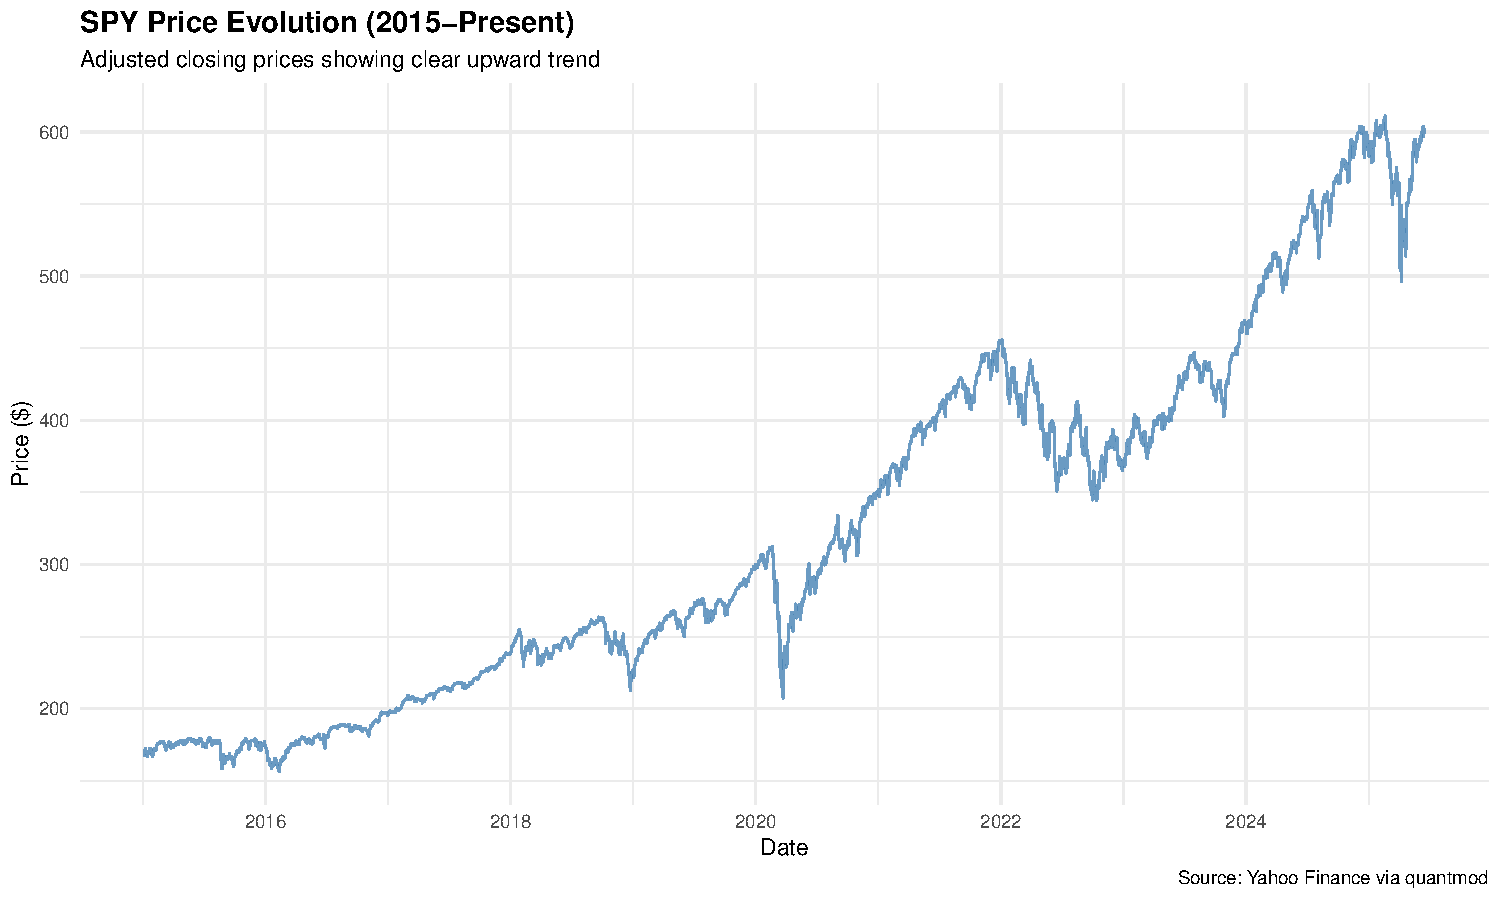
\includegraphics{task1_files/figure-latex/return-analysis-plots-1.pdf}

\begin{Shaded}
\begin{Highlighting}[]
\NormalTok{plots}\SpecialCharTok{$}\NormalTok{return\_hist}
\end{Highlighting}
\end{Shaded}

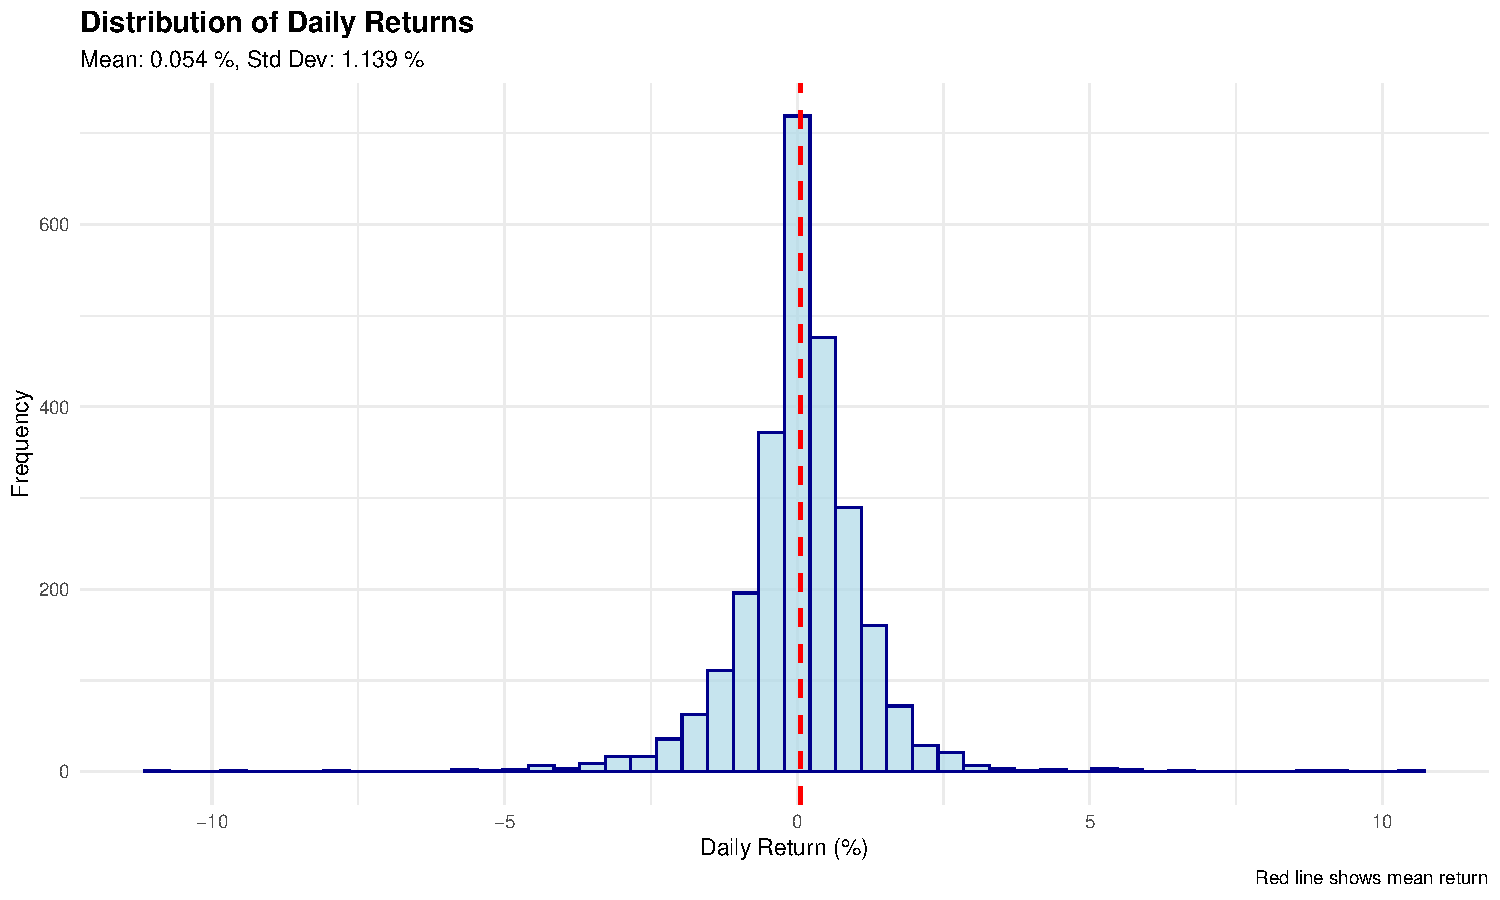
\includegraphics{task1_files/figure-latex/return-analysis-plots-2.pdf}

\begin{Shaded}
\begin{Highlighting}[]
\NormalTok{plots}\SpecialCharTok{$}\NormalTok{return\_ts}
\end{Highlighting}
\end{Shaded}

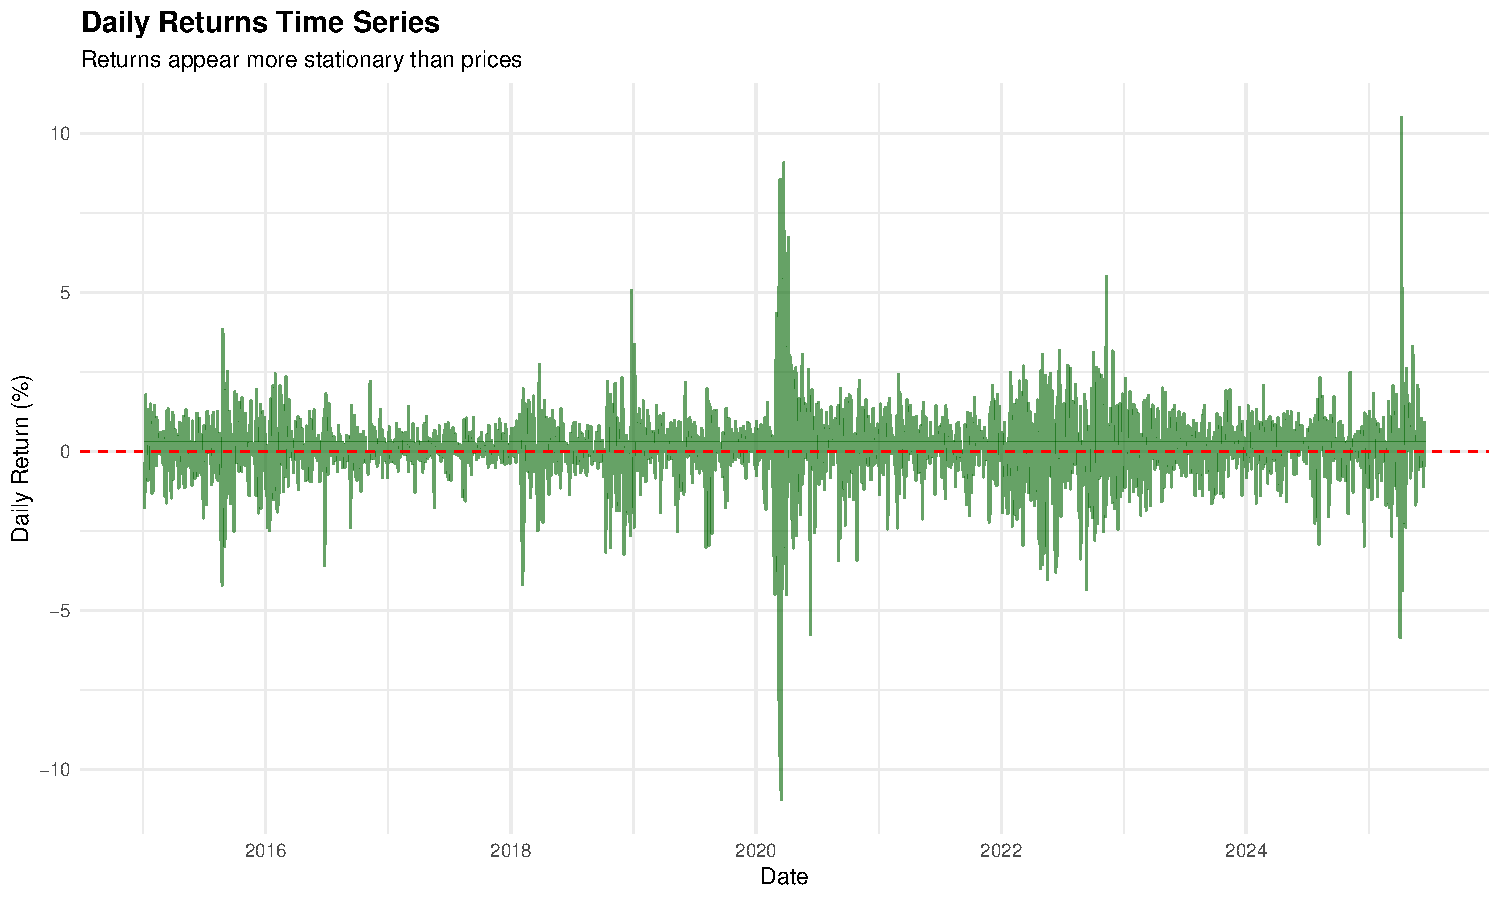
\includegraphics{task1_files/figure-latex/return-analysis-plots-3.pdf}

\begin{Shaded}
\begin{Highlighting}[]
\CommentTok{\# Domain Service: Statistical Analysis}
\CommentTok{\# Responsibility: Provide comprehensive return statistics}
\NormalTok{analyze\_return\_properties }\OtherTok{\textless{}{-}} \ControlFlowTok{function}\NormalTok{(return\_data) \{}
  \CommentTok{\# Basic statistics}
\NormalTok{  basic\_stats }\OtherTok{\textless{}{-}}\NormalTok{ return\_data }\SpecialCharTok{\%\textgreater{}\%}
    \FunctionTok{summarise}\NormalTok{(}
      \AttributeTok{observations =} \FunctionTok{n}\NormalTok{(),}
      \AttributeTok{mean\_return =} \FunctionTok{mean}\NormalTok{(return\_pct),}
      \AttributeTok{std\_dev =} \FunctionTok{sd}\NormalTok{(return\_pct),}
      \AttributeTok{min\_return =} \FunctionTok{min}\NormalTok{(return\_pct),}
      \AttributeTok{max\_return =} \FunctionTok{max}\NormalTok{(return\_pct),}
      \AttributeTok{skewness =}\NormalTok{ moments}\SpecialCharTok{::}\FunctionTok{skewness}\NormalTok{(return\_pct),}
      \AttributeTok{kurtosis =}\NormalTok{ moments}\SpecialCharTok{::}\FunctionTok{kurtosis}\NormalTok{(return\_pct),}
      \AttributeTok{.groups =} \StringTok{"drop"}
\NormalTok{    )}
  
  \CommentTok{\# Annualized statistics (assuming 252 trading days per year)}
\NormalTok{  annualized\_stats }\OtherTok{\textless{}{-}} \FunctionTok{list}\NormalTok{(}
    \AttributeTok{annual\_mean =}\NormalTok{ basic\_stats}\SpecialCharTok{$}\NormalTok{mean\_return }\SpecialCharTok{*} \DecValTok{252}\NormalTok{,}
    \AttributeTok{annual\_volatility =}\NormalTok{ basic\_stats}\SpecialCharTok{$}\NormalTok{std\_dev }\SpecialCharTok{*} \FunctionTok{sqrt}\NormalTok{(}\DecValTok{252}\NormalTok{),}
    \AttributeTok{sharpe\_ratio =}\NormalTok{ (basic\_stats}\SpecialCharTok{$}\NormalTok{mean\_return }\SpecialCharTok{*} \DecValTok{252}\NormalTok{) }\SpecialCharTok{/}\NormalTok{ (basic\_stats}\SpecialCharTok{$}\NormalTok{std\_dev }\SpecialCharTok{*} \FunctionTok{sqrt}\NormalTok{(}\DecValTok{252}\NormalTok{))}
\NormalTok{  )}
  
  \FunctionTok{cat}\NormalTok{(}\StringTok{"=== RETURN ANALYSIS SUMMARY ===}\SpecialCharTok{\textbackslash{}n\textbackslash{}n}\StringTok{"}\NormalTok{)}
  \FunctionTok{cat}\NormalTok{(}\StringTok{"Daily Statistics:}\SpecialCharTok{\textbackslash{}n}\StringTok{"}\NormalTok{)}
  \FunctionTok{cat}\NormalTok{(}\StringTok{"  Mean Return:"}\NormalTok{, }\FunctionTok{sprintf}\NormalTok{(}\StringTok{"\%.4f\%\%"}\NormalTok{, basic\_stats}\SpecialCharTok{$}\NormalTok{mean\_return), }\StringTok{"}\SpecialCharTok{\textbackslash{}n}\StringTok{"}\NormalTok{)}
  \FunctionTok{cat}\NormalTok{(}\StringTok{"  Volatility: "}\NormalTok{, }\FunctionTok{sprintf}\NormalTok{(}\StringTok{"\%.4f\%\%"}\NormalTok{, basic\_stats}\SpecialCharTok{$}\NormalTok{std\_dev), }\StringTok{"}\SpecialCharTok{\textbackslash{}n}\StringTok{"}\NormalTok{)}
  \FunctionTok{cat}\NormalTok{(}\StringTok{"  Min Return: "}\NormalTok{, }\FunctionTok{sprintf}\NormalTok{(}\StringTok{"\%.2f\%\%"}\NormalTok{, basic\_stats}\SpecialCharTok{$}\NormalTok{min\_return), }\StringTok{"}\SpecialCharTok{\textbackslash{}n}\StringTok{"}\NormalTok{)}
  \FunctionTok{cat}\NormalTok{(}\StringTok{"  Max Return: "}\NormalTok{, }\FunctionTok{sprintf}\NormalTok{(}\StringTok{"\%.2f\%\%"}\NormalTok{, basic\_stats}\SpecialCharTok{$}\NormalTok{max\_return), }\StringTok{"}\SpecialCharTok{\textbackslash{}n}\StringTok{"}\NormalTok{)}
  \FunctionTok{cat}\NormalTok{(}\StringTok{"  Skewness:    "}\NormalTok{, }\FunctionTok{sprintf}\NormalTok{(}\StringTok{"\%.4f"}\NormalTok{, basic\_stats}\SpecialCharTok{$}\NormalTok{skewness), }\StringTok{"}\SpecialCharTok{\textbackslash{}n}\StringTok{"}\NormalTok{)}
  \FunctionTok{cat}\NormalTok{(}\StringTok{"  Kurtosis:    "}\NormalTok{, }\FunctionTok{sprintf}\NormalTok{(}\StringTok{"\%.4f"}\NormalTok{, basic\_stats}\SpecialCharTok{$}\NormalTok{kurtosis), }\StringTok{"}\SpecialCharTok{\textbackslash{}n\textbackslash{}n}\StringTok{"}\NormalTok{)}
  
  \FunctionTok{cat}\NormalTok{(}\StringTok{"Annualized Statistics:}\SpecialCharTok{\textbackslash{}n}\StringTok{"}\NormalTok{)}
  \FunctionTok{cat}\NormalTok{(}\StringTok{"  Annual Return:"}\NormalTok{, }\FunctionTok{sprintf}\NormalTok{(}\StringTok{"\%.2f\%\%"}\NormalTok{, annualized\_stats}\SpecialCharTok{$}\NormalTok{annual\_mean), }\StringTok{"}\SpecialCharTok{\textbackslash{}n}\StringTok{"}\NormalTok{)}
  \FunctionTok{cat}\NormalTok{(}\StringTok{"  Annual Vol:    "}\NormalTok{, }\FunctionTok{sprintf}\NormalTok{(}\StringTok{"\%.2f\%\%"}\NormalTok{, annualized\_stats}\SpecialCharTok{$}\NormalTok{annual\_volatility), }\StringTok{"}\SpecialCharTok{\textbackslash{}n}\StringTok{"}\NormalTok{)}
  \FunctionTok{cat}\NormalTok{(}\StringTok{"  Sharpe Ratio: "}\NormalTok{, }\FunctionTok{sprintf}\NormalTok{(}\StringTok{"\%.4f"}\NormalTok{, annualized\_stats}\SpecialCharTok{$}\NormalTok{sharpe\_ratio), }\StringTok{"}\SpecialCharTok{\textbackslash{}n\textbackslash{}n}\StringTok{"}\NormalTok{)}
  
  \FunctionTok{return}\NormalTok{(}\FunctionTok{list}\NormalTok{(}
    \AttributeTok{daily =}\NormalTok{ basic\_stats,}
    \AttributeTok{annual =}\NormalTok{ annualized\_stats}
\NormalTok{  ))}
\NormalTok{\}}

\CommentTok{\# Perform return analysis}
\NormalTok{return\_analysis }\OtherTok{\textless{}{-}} \FunctionTok{analyze\_return\_properties}\NormalTok{(spy\_returns)}
\end{Highlighting}
\end{Shaded}

\begin{verbatim}
## === RETURN ANALYSIS SUMMARY ===
## 
## Daily Statistics:
##   Mean Return: 0.0542% 
##   Volatility:  1.1392% 
##   Min Return:  -10.94% 
##   Max Return:  10.50% 
##   Skewness:     -0.3015 
##   Kurtosis:     16.8614 
## 
## Annualized Statistics:
##   Annual Return: 13.66% 
##   Annual Vol:     18.08% 
##   Sharpe Ratio:  0.7554
\end{verbatim}

\hypertarget{exercise-3-state-vector-implementation}{%
\section{Exercise 3: State Vector
Implementation}\label{exercise-3-state-vector-implementation}}

\hypertarget{state-vector-concept}{%
\subsection{State Vector Concept}\label{state-vector-concept}}

According to our glossary, a \textbf{State} represents ``all the
information the agent sees right now when deciding.'' In our trading
context, this is a window of recent returns that should satisfy the
\textbf{Markov property} - containing sufficient information to predict
what happens next.

\begin{Shaded}
\begin{Highlighting}[]
\CommentTok{\# Domain Entity: State Vector Factory}
\CommentTok{\# Responsibility: Encapsulate the current market state for agent decision{-}making}
\NormalTok{create\_state\_vector\_factory }\OtherTok{\textless{}{-}} \ControlFlowTok{function}\NormalTok{(}\AttributeTok{window\_size =} \DecValTok{10}\NormalTok{) \{}
  \CommentTok{\# Validate window size}
  \ControlFlowTok{if}\NormalTok{ (}\SpecialCharTok{!}\FunctionTok{is.numeric}\NormalTok{(window\_size) }\SpecialCharTok{||}\NormalTok{ window\_size }\SpecialCharTok{\textless{}=} \DecValTok{0} \SpecialCharTok{||}\NormalTok{ window\_size }\SpecialCharTok{!=} \FunctionTok{as.integer}\NormalTok{(window\_size)) \{}
    \FunctionTok{stop}\NormalTok{(}\StringTok{"window\_size must be a positive integer"}\NormalTok{)}
\NormalTok{  \}}
  
  \CommentTok{\# Return factory function that creates state vectors}
  \ControlFlowTok{function}\NormalTok{(return\_data, t\_index) \{}
    \CommentTok{\# Input validation}
    \ControlFlowTok{if}\NormalTok{ (}\SpecialCharTok{!}\FunctionTok{is.data.frame}\NormalTok{(return\_data) }\SpecialCharTok{||} \SpecialCharTok{!}\StringTok{"return\_pct"} \SpecialCharTok{\%in\%} \FunctionTok{names}\NormalTok{(return\_data)) \{}
      \FunctionTok{stop}\NormalTok{(}\StringTok{"return\_data must be a data frame with \textquotesingle{}return\_pct\textquotesingle{} column"}\NormalTok{)}
\NormalTok{    \}}
    
    \ControlFlowTok{if}\NormalTok{ (}\SpecialCharTok{!}\FunctionTok{is.numeric}\NormalTok{(t\_index) }\SpecialCharTok{||} \FunctionTok{length}\NormalTok{(t\_index) }\SpecialCharTok{!=} \DecValTok{1}\NormalTok{) \{}
      \FunctionTok{stop}\NormalTok{(}\StringTok{"t\_index must be a single numeric value"}\NormalTok{)}
\NormalTok{    \}}
    
    \CommentTok{\# Check if we have enough data to create the window}
    \ControlFlowTok{if}\NormalTok{ (t\_index }\SpecialCharTok{\textless{}}\NormalTok{ window\_size) \{}
      \FunctionTok{stop}\NormalTok{(}\FunctionTok{paste}\NormalTok{(}\StringTok{"t\_index must be at least"}\NormalTok{, window\_size, }
                 \StringTok{"to create a window of size"}\NormalTok{, window\_size))}
\NormalTok{    \}}
    
    \ControlFlowTok{if}\NormalTok{ (t\_index }\SpecialCharTok{\textgreater{}} \FunctionTok{nrow}\NormalTok{(return\_data)) \{}
      \FunctionTok{stop}\NormalTok{(}\FunctionTok{paste}\NormalTok{(}\StringTok{"t\_index cannot exceed the number of observations:"}\NormalTok{, }\FunctionTok{nrow}\NormalTok{(return\_data)))}
\NormalTok{    \}}
    
    \CommentTok{\# Calculate window boundaries}
    \CommentTok{\# For t\_index = 15 and window\_size = 10, we want observations 6{-}15}
\NormalTok{    start\_idx }\OtherTok{\textless{}{-}}\NormalTok{ t\_index }\SpecialCharTok{{-}}\NormalTok{ window\_size }\SpecialCharTok{+} \DecValTok{1}
\NormalTok{    end\_idx }\OtherTok{\textless{}{-}}\NormalTok{ t\_index}
    
    \CommentTok{\# Extract the state vector}
\NormalTok{    state\_vector }\OtherTok{\textless{}{-}}\NormalTok{ return\_data}\SpecialCharTok{$}\NormalTok{return\_pct[start\_idx}\SpecialCharTok{:}\NormalTok{end\_idx]}
    
    \CommentTok{\# Create metadata for the state}
\NormalTok{    state\_metadata }\OtherTok{\textless{}{-}} \FunctionTok{list}\NormalTok{(}
      \AttributeTok{t\_index =}\NormalTok{ t\_index,}
      \AttributeTok{window\_size =}\NormalTok{ window\_size,}
      \AttributeTok{start\_idx =}\NormalTok{ start\_idx,}
      \AttributeTok{end\_idx =}\NormalTok{ end\_idx,}
      \AttributeTok{date\_range =} \FunctionTok{c}\NormalTok{(}
\NormalTok{        return\_data}\SpecialCharTok{$}\NormalTok{date[start\_idx],}
\NormalTok{        return\_data}\SpecialCharTok{$}\NormalTok{date[end\_idx]}
\NormalTok{      )}
\NormalTok{    )}
    
    \CommentTok{\# Return state object with data and metadata}
    \FunctionTok{structure}\NormalTok{(}
      \FunctionTok{list}\NormalTok{(}
        \AttributeTok{values =}\NormalTok{ state\_vector,}
        \AttributeTok{metadata =}\NormalTok{ state\_metadata}
\NormalTok{      ),}
      \AttributeTok{class =} \StringTok{"MarketState"}
\NormalTok{    )}
\NormalTok{  \}}
\NormalTok{\}}

\CommentTok{\# Create the state vector factory with window size 10}
\NormalTok{make\_state }\OtherTok{\textless{}{-}} \FunctionTok{create\_state\_vector\_factory}\NormalTok{(}\AttributeTok{window\_size =} \DecValTok{10}\NormalTok{)}

\CommentTok{\# Test the implementation with the required example: t = 15 should look at bars 6{-}15}
\NormalTok{test\_state }\OtherTok{\textless{}{-}} \FunctionTok{make\_state}\NormalTok{(spy\_returns, }\AttributeTok{t\_index =} \DecValTok{15}\NormalTok{)}

\FunctionTok{cat}\NormalTok{(}\StringTok{"=== STATE VECTOR TEST (t\_index = 15) ===}\SpecialCharTok{\textbackslash{}n\textbackslash{}n}\StringTok{"}\NormalTok{)}
\end{Highlighting}
\end{Shaded}

\begin{verbatim}
## === STATE VECTOR TEST (t_index = 15) ===
\end{verbatim}

\begin{Shaded}
\begin{Highlighting}[]
\FunctionTok{cat}\NormalTok{(}\StringTok{"Expected: observations 6{-}15 (indices"}\NormalTok{, }\DecValTok{6}\NormalTok{, }\StringTok{"to"}\NormalTok{, }\DecValTok{15}\NormalTok{, }\StringTok{")}\SpecialCharTok{\textbackslash{}n}\StringTok{"}\NormalTok{)}
\end{Highlighting}
\end{Shaded}

\begin{verbatim}
## Expected: observations 6-15 (indices 6 to 15 )
\end{verbatim}

\begin{Shaded}
\begin{Highlighting}[]
\FunctionTok{cat}\NormalTok{(}\StringTok{"Actual:    observations"}\NormalTok{, test\_state}\SpecialCharTok{$}\NormalTok{metadata}\SpecialCharTok{$}\NormalTok{start\_idx, }\StringTok{"to"}\NormalTok{, test\_state}\SpecialCharTok{$}\NormalTok{metadata}\SpecialCharTok{$}\NormalTok{end\_idx, }\StringTok{"}\SpecialCharTok{\textbackslash{}n}\StringTok{"}\NormalTok{)}
\end{Highlighting}
\end{Shaded}

\begin{verbatim}
## Actual:    observations 6 to 15
\end{verbatim}

\begin{Shaded}
\begin{Highlighting}[]
\FunctionTok{cat}\NormalTok{(}\StringTok{"Window size:"}\NormalTok{, test\_state}\SpecialCharTok{$}\NormalTok{metadata}\SpecialCharTok{$}\NormalTok{window\_size, }\StringTok{"}\SpecialCharTok{\textbackslash{}n}\StringTok{"}\NormalTok{)}
\end{Highlighting}
\end{Shaded}

\begin{verbatim}
## Window size: 10
\end{verbatim}

\begin{Shaded}
\begin{Highlighting}[]
\FunctionTok{cat}\NormalTok{(}\StringTok{"Date range:"}\NormalTok{, }\FunctionTok{as.character}\NormalTok{(test\_state}\SpecialCharTok{$}\NormalTok{metadata}\SpecialCharTok{$}\NormalTok{date\_range[}\DecValTok{1}\NormalTok{]), }\StringTok{"to"}\NormalTok{, }
    \FunctionTok{as.character}\NormalTok{(test\_state}\SpecialCharTok{$}\NormalTok{metadata}\SpecialCharTok{$}\NormalTok{date\_range[}\DecValTok{2}\NormalTok{]), }\StringTok{"}\SpecialCharTok{\textbackslash{}n\textbackslash{}n}\StringTok{"}\NormalTok{)}
\end{Highlighting}
\end{Shaded}

\begin{verbatim}
## Date range: 2015-01-12 to 2015-01-26
\end{verbatim}

\begin{Shaded}
\begin{Highlighting}[]
\FunctionTok{cat}\NormalTok{(}\StringTok{"State vector values:}\SpecialCharTok{\textbackslash{}n}\StringTok{"}\NormalTok{)}
\end{Highlighting}
\end{Shaded}

\begin{verbatim}
## State vector values:
\end{verbatim}

\begin{Shaded}
\begin{Highlighting}[]
\FunctionTok{print}\NormalTok{(}\FunctionTok{round}\NormalTok{(test\_state}\SpecialCharTok{$}\NormalTok{values, }\DecValTok{4}\NormalTok{))}
\end{Highlighting}
\end{Shaded}

\begin{verbatim}
##  [1] -0.7834 -0.2813 -0.6037 -0.9161  1.3114  0.2133  0.5048  1.4871 -0.5483
## [10]  0.2342
\end{verbatim}

\begin{Shaded}
\begin{Highlighting}[]
\CommentTok{\# Verify our implementation matches the specification}
\NormalTok{verification\_passed }\OtherTok{\textless{}{-}}\NormalTok{ (test\_state}\SpecialCharTok{$}\NormalTok{metadata}\SpecialCharTok{$}\NormalTok{start\_idx }\SpecialCharTok{==} \DecValTok{6} \SpecialCharTok{\&\&}\NormalTok{ test\_state}\SpecialCharTok{$}\NormalTok{metadata}\SpecialCharTok{$}\NormalTok{end\_idx }\SpecialCharTok{==} \DecValTok{15}\NormalTok{)}
\FunctionTok{cat}\NormalTok{(}\StringTok{"}\SpecialCharTok{\textbackslash{}n}\StringTok{Verification:"}\NormalTok{, }\FunctionTok{ifelse}\NormalTok{(verification\_passed, }\StringTok{"PASSED ✓"}\NormalTok{, }\StringTok{"FAILED ✗"}\NormalTok{), }\StringTok{"}\SpecialCharTok{\textbackslash{}n}\StringTok{"}\NormalTok{)}
\end{Highlighting}
\end{Shaded}

\begin{verbatim}
## 
## Verification: PASSED ✓
\end{verbatim}

\begin{Shaded}
\begin{Highlighting}[]
\CommentTok{\# Domain Service: State Vector Validator}
\CommentTok{\# Responsibility: Ensure state vectors meet quality requirements}
\NormalTok{validate\_state\_vector }\OtherTok{\textless{}{-}} \ControlFlowTok{function}\NormalTok{(state\_obj) \{}
  \CommentTok{\# Check if it\textquotesingle{}s a proper MarketState object}
  \ControlFlowTok{if}\NormalTok{ (}\SpecialCharTok{!}\FunctionTok{inherits}\NormalTok{(state\_obj, }\StringTok{"MarketState"}\NormalTok{)) \{}
    \FunctionTok{return}\NormalTok{(}\FunctionTok{list}\NormalTok{(}\AttributeTok{valid =} \ConstantTok{FALSE}\NormalTok{, }\AttributeTok{message =} \StringTok{"Not a MarketState object"}\NormalTok{))}
\NormalTok{  \}}
  
  \CommentTok{\# Check if values are numeric and finite}
  \ControlFlowTok{if}\NormalTok{ (}\SpecialCharTok{!}\FunctionTok{is.numeric}\NormalTok{(state\_obj}\SpecialCharTok{$}\NormalTok{values) }\SpecialCharTok{||} \FunctionTok{any}\NormalTok{(}\SpecialCharTok{!}\FunctionTok{is.finite}\NormalTok{(state\_obj}\SpecialCharTok{$}\NormalTok{values))) \{}
    \FunctionTok{return}\NormalTok{(}\FunctionTok{list}\NormalTok{(}\AttributeTok{valid =} \ConstantTok{FALSE}\NormalTok{, }\AttributeTok{message =} \StringTok{"State values must be finite numbers"}\NormalTok{))}
\NormalTok{  \}}
  
  \CommentTok{\# Check window size consistency}
\NormalTok{  expected\_length }\OtherTok{\textless{}{-}}\NormalTok{ state\_obj}\SpecialCharTok{$}\NormalTok{metadata}\SpecialCharTok{$}\NormalTok{window\_size}
\NormalTok{  actual\_length }\OtherTok{\textless{}{-}} \FunctionTok{length}\NormalTok{(state\_obj}\SpecialCharTok{$}\NormalTok{values)}
  
  \ControlFlowTok{if}\NormalTok{ (actual\_length }\SpecialCharTok{!=}\NormalTok{ expected\_length) \{}
    \FunctionTok{return}\NormalTok{(}\FunctionTok{list}\NormalTok{(}\AttributeTok{valid =} \ConstantTok{FALSE}\NormalTok{, }
                \AttributeTok{message =} \FunctionTok{paste}\NormalTok{(}\StringTok{"Length mismatch: expected"}\NormalTok{, expected\_length, }
                                \StringTok{"got"}\NormalTok{, actual\_length)))}
\NormalTok{  \}}
  
  \FunctionTok{return}\NormalTok{(}\FunctionTok{list}\NormalTok{(}\AttributeTok{valid =} \ConstantTok{TRUE}\NormalTok{, }\AttributeTok{message =} \StringTok{"State vector is valid"}\NormalTok{))}
\NormalTok{\}}

\CommentTok{\# Validate our test state}
\NormalTok{validation\_result }\OtherTok{\textless{}{-}} \FunctionTok{validate\_state\_vector}\NormalTok{(test\_state)}
\FunctionTok{cat}\NormalTok{(}\StringTok{"State validation:"}\NormalTok{, validation\_result}\SpecialCharTok{$}\NormalTok{message, }\StringTok{"}\SpecialCharTok{\textbackslash{}n}\StringTok{"}\NormalTok{)}
\end{Highlighting}
\end{Shaded}

\begin{verbatim}
## State validation: State vector is valid
\end{verbatim}

\begin{Shaded}
\begin{Highlighting}[]
\CommentTok{\# Demonstrate creating multiple states}
\FunctionTok{cat}\NormalTok{(}\StringTok{"}\SpecialCharTok{\textbackslash{}n}\StringTok{=== MULTIPLE STATE VECTOR EXAMPLES ===}\SpecialCharTok{\textbackslash{}n}\StringTok{"}\NormalTok{)}
\end{Highlighting}
\end{Shaded}

\begin{verbatim}
## 
## === MULTIPLE STATE VECTOR EXAMPLES ===
\end{verbatim}

\begin{Shaded}
\begin{Highlighting}[]
\CommentTok{\# Create several state vectors to show the sliding window concept}
\NormalTok{example\_indices }\OtherTok{\textless{}{-}} \FunctionTok{c}\NormalTok{(}\DecValTok{20}\NormalTok{, }\DecValTok{50}\NormalTok{, }\DecValTok{100}\NormalTok{, }\DecValTok{200}\NormalTok{)}

\ControlFlowTok{for}\NormalTok{ (idx }\ControlFlowTok{in}\NormalTok{ example\_indices) \{}
  \ControlFlowTok{if}\NormalTok{ (idx }\SpecialCharTok{\textless{}=} \FunctionTok{nrow}\NormalTok{(spy\_returns)) \{}
\NormalTok{    state }\OtherTok{\textless{}{-}} \FunctionTok{make\_state}\NormalTok{(spy\_returns, idx)}
    \FunctionTok{cat}\NormalTok{(}\StringTok{"}\SpecialCharTok{\textbackslash{}n}\StringTok{State at t ="}\NormalTok{, idx, }\StringTok{":}\SpecialCharTok{\textbackslash{}n}\StringTok{"}\NormalTok{)}
    \FunctionTok{cat}\NormalTok{(}\StringTok{"  Date:"}\NormalTok{, }\FunctionTok{as.character}\NormalTok{(state}\SpecialCharTok{$}\NormalTok{metadata}\SpecialCharTok{$}\NormalTok{date\_range[}\DecValTok{2}\NormalTok{]), }\StringTok{"}\SpecialCharTok{\textbackslash{}n}\StringTok{"}\NormalTok{)}
    \FunctionTok{cat}\NormalTok{(}\StringTok{"  Window:"}\NormalTok{, state}\SpecialCharTok{$}\NormalTok{metadata}\SpecialCharTok{$}\NormalTok{start\_idx, }\StringTok{"to"}\NormalTok{, state}\SpecialCharTok{$}\NormalTok{metadata}\SpecialCharTok{$}\NormalTok{end\_idx, }\StringTok{"}\SpecialCharTok{\textbackslash{}n}\StringTok{"}\NormalTok{)}
    \FunctionTok{cat}\NormalTok{(}\StringTok{"  Mean return in window:"}\NormalTok{, }\FunctionTok{round}\NormalTok{(}\FunctionTok{mean}\NormalTok{(state}\SpecialCharTok{$}\NormalTok{values), }\DecValTok{4}\NormalTok{), }\StringTok{"\%}\SpecialCharTok{\textbackslash{}n}\StringTok{"}\NormalTok{)}
    \FunctionTok{cat}\NormalTok{(}\StringTok{"  Std dev in window:"}\NormalTok{, }\FunctionTok{round}\NormalTok{(}\FunctionTok{sd}\NormalTok{(state}\SpecialCharTok{$}\NormalTok{values), }\DecValTok{4}\NormalTok{), }\StringTok{"\%}\SpecialCharTok{\textbackslash{}n}\StringTok{"}\NormalTok{)}
\NormalTok{  \}}
\NormalTok{\}}
\end{Highlighting}
\end{Shaded}

\begin{verbatim}
## 
## State at t = 20 :
##   Date: 2015-02-02 
##   Window: 11 to 20 
##   Mean return in window: 0.0195 %
##   Std dev in window: 1.0655 %
## 
## State at t = 50 :
##   Date: 2015-03-17 
##   Window: 41 to 50 
##   Mean return in window: -0.1464 %
##   Std dev in window: 0.9819 %
## 
## State at t = 100 :
##   Date: 2015-05-28 
##   Window: 91 to 100 
##   Mean return in window: 0.1172 %
##   Std dev in window: 0.6033 %
## 
## State at t = 200 :
##   Date: 2015-10-19 
##   Window: 191 to 200 
##   Mean return in window: 0.2463 %
##   Std dev in window: 0.6834 %
\end{verbatim}

\begin{Shaded}
\begin{Highlighting}[]
\CommentTok{\# Domain Service: State Visualization}
\CommentTok{\# Responsibility: Provide visual understanding of state vectors}
\NormalTok{visualize\_state\_vector }\OtherTok{\textless{}{-}} \ControlFlowTok{function}\NormalTok{(return\_data, t\_index, }\AttributeTok{window\_size =} \DecValTok{10}\NormalTok{) \{}
  \CommentTok{\# Create state for visualization}
\NormalTok{  state }\OtherTok{\textless{}{-}} \FunctionTok{make\_state}\NormalTok{(return\_data, t\_index)}
  
  \CommentTok{\# Prepare data for plotting}
\NormalTok{  plot\_data }\OtherTok{\textless{}{-}}\NormalTok{ return\_data }\SpecialCharTok{\%\textgreater{}\%}
    \FunctionTok{mutate}\NormalTok{(}
      \AttributeTok{index =} \FunctionTok{row\_number}\NormalTok{(),}
      \AttributeTok{in\_window =}\NormalTok{ index }\SpecialCharTok{\textgreater{}=}\NormalTok{ state}\SpecialCharTok{$}\NormalTok{metadata}\SpecialCharTok{$}\NormalTok{start\_idx }\SpecialCharTok{\&}\NormalTok{ index }\SpecialCharTok{\textless{}=}\NormalTok{ state}\SpecialCharTok{$}\NormalTok{metadata}\SpecialCharTok{$}\NormalTok{end\_idx,}
      \AttributeTok{is\_current =}\NormalTok{ index }\SpecialCharTok{==}\NormalTok{ t\_index,}
      \CommentTok{\# Create a new categorical variable for coloring and sizing points}
      \AttributeTok{point\_type =} \FunctionTok{case\_when}\NormalTok{(}
\NormalTok{        is\_current }\SpecialCharTok{\textasciitilde{}} \StringTok{"Current"}\NormalTok{,}
\NormalTok{        in\_window }\SpecialCharTok{\textasciitilde{}} \StringTok{"In Window"}\NormalTok{,}
        \ConstantTok{TRUE} \SpecialCharTok{\textasciitilde{}} \StringTok{"Outside"}
\NormalTok{      )}
\NormalTok{    ) }\SpecialCharTok{\%\textgreater{}\%}
    \FunctionTok{filter}\NormalTok{(index }\SpecialCharTok{\textgreater{}=}\NormalTok{ (t\_index }\SpecialCharTok{{-}} \DecValTok{20}\NormalTok{) }\SpecialCharTok{\&}\NormalTok{ index }\SpecialCharTok{\textless{}=}\NormalTok{ (t\_index }\SpecialCharTok{+} \DecValTok{5}\NormalTok{))  }\CommentTok{\# Show context around the window}
  
  \CommentTok{\# Create the plot}
  \FunctionTok{ggplot}\NormalTok{(plot\_data, }\FunctionTok{aes}\NormalTok{(}\AttributeTok{x =}\NormalTok{ index, }\AttributeTok{y =}\NormalTok{ return\_pct)) }\SpecialCharTok{+}
    \FunctionTok{geom\_line}\NormalTok{(}\AttributeTok{color =} \StringTok{"lightgray"}\NormalTok{, }\AttributeTok{alpha =} \FloatTok{0.5}\NormalTok{) }\SpecialCharTok{+}
    \FunctionTok{geom\_point}\NormalTok{(}\FunctionTok{aes}\NormalTok{(}\AttributeTok{color =}\NormalTok{ point\_type, }\AttributeTok{size =}\NormalTok{ point\_type)) }\SpecialCharTok{+}
    \FunctionTok{scale\_color\_manual}\NormalTok{(}
      \AttributeTok{name =} \StringTok{"State"}\NormalTok{,}
      \AttributeTok{values =} \FunctionTok{c}\NormalTok{(}\StringTok{"In Window"} \OtherTok{=} \StringTok{"steelblue"}\NormalTok{, }
                 \StringTok{"Current"} \OtherTok{=} \StringTok{"red"}\NormalTok{, }
                 \StringTok{"Outside"} \OtherTok{=} \StringTok{"lightgray"}\NormalTok{)}
\NormalTok{    ) }\SpecialCharTok{+}
    \FunctionTok{scale\_size\_manual}\NormalTok{(}
      \AttributeTok{name =} \StringTok{"State"}\NormalTok{,}
      \AttributeTok{values =} \FunctionTok{c}\NormalTok{(}\StringTok{"In Window"} \OtherTok{=} \DecValTok{2}\NormalTok{, }
                 \StringTok{"Current"} \OtherTok{=} \DecValTok{3}\NormalTok{, }
                 \StringTok{"Outside"} \OtherTok{=} \DecValTok{1}\NormalTok{)}
\NormalTok{    ) }\SpecialCharTok{+}
    \FunctionTok{labs}\NormalTok{(}
      \AttributeTok{title =} \FunctionTok{paste}\NormalTok{(}\StringTok{"State Vector Visualization (t ="}\NormalTok{, t\_index, }\StringTok{")"}\NormalTok{),}
      \AttributeTok{subtitle =} \FunctionTok{paste}\NormalTok{(}\StringTok{"Window size:"}\NormalTok{, window\_size, }\StringTok{"| Observations"}\NormalTok{, }
\NormalTok{                       state}\SpecialCharTok{$}\NormalTok{metadata}\SpecialCharTok{$}\NormalTok{start\_idx, }\StringTok{"to"}\NormalTok{, state}\SpecialCharTok{$}\NormalTok{metadata}\SpecialCharTok{$}\NormalTok{end\_idx),}
      \AttributeTok{x =} \StringTok{"Observation Index"}\NormalTok{,}
      \AttributeTok{y =} \StringTok{"Return (\%)"}\NormalTok{,}
      \AttributeTok{caption =} \StringTok{"Red point = current time, Blue points = state window"}
\NormalTok{    ) }\SpecialCharTok{+}
    \FunctionTok{theme\_minimal}\NormalTok{() }\SpecialCharTok{+}
    \FunctionTok{theme}\NormalTok{(}
      \AttributeTok{plot.title =} \FunctionTok{element\_text}\NormalTok{(}\AttributeTok{size =} \DecValTok{14}\NormalTok{, }\AttributeTok{face =} \StringTok{"bold"}\NormalTok{),}
      \AttributeTok{legend.position =} \StringTok{"bottom"}
\NormalTok{    )}
\NormalTok{\}}

\CommentTok{\# Visualize the test state}
\NormalTok{state\_plot }\OtherTok{\textless{}{-}} \FunctionTok{visualize\_state\_vector}\NormalTok{(spy\_returns, }\AttributeTok{t\_index =} \DecValTok{15}\NormalTok{)}
\NormalTok{state\_plot}
\end{Highlighting}
\end{Shaded}

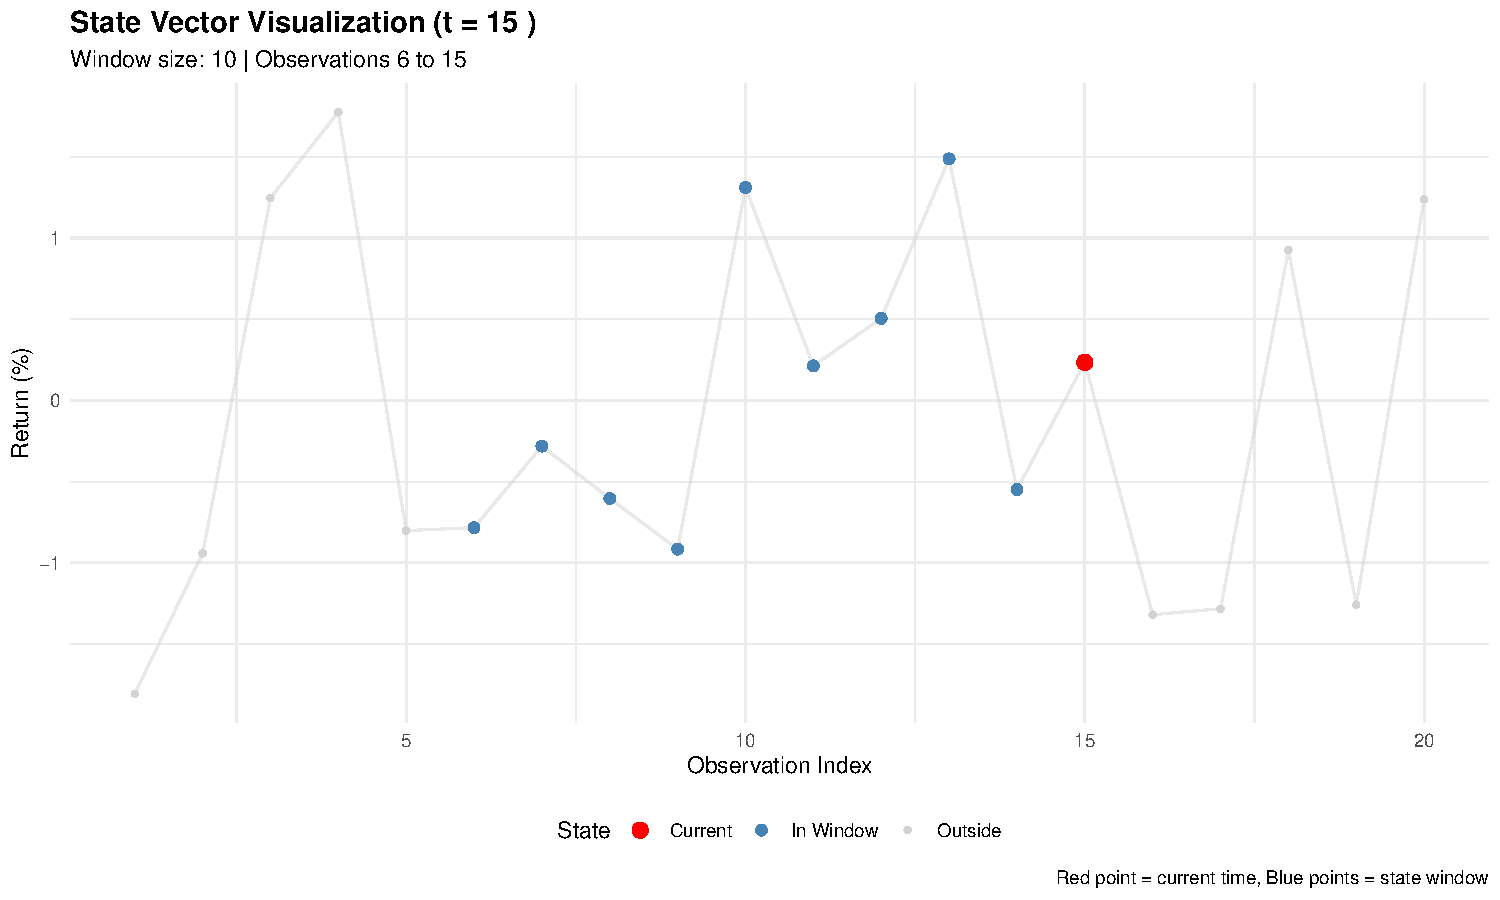
\includegraphics{task1_files/figure-latex/state-visualization-1.pdf}

\hypertarget{exercise-4-neural-network-setup}{%
\section{Exercise 4: Neural Network
Setup}\label{exercise-4-neural-network-setup}}

Our Q-network will approximate the optimal Q-values for each action
given a specific state. The input to the network will be the state
vector (e.g., 10 recent returns), and the output will be the Q-values
for each possible action (e.g., Buy, Sell, Hold).

\begin{Shaded}
\begin{Highlighting}[]
\CommentTok{\# Define actions available to the agent}
\CommentTok{\# Domain Entity: Action}
\CommentTok{\# Responsibility: Define possible actions for the agent}
\NormalTok{ACTIONS }\OtherTok{\textless{}{-}} \FunctionTok{c}\NormalTok{(}\StringTok{"Buy"}\NormalTok{, }\StringTok{"Sell"}\NormalTok{, }\StringTok{"Hold"}\NormalTok{)}
\NormalTok{NUM\_ACTIONS }\OtherTok{\textless{}{-}} \FunctionTok{length}\NormalTok{(ACTIONS)}

\CommentTok{\# Domain Service: Q{-}Network Factory}
\CommentTok{\# Responsibility: Create and manage the neural network architecture}
\NormalTok{create\_q\_network }\OtherTok{\textless{}{-}} \ControlFlowTok{function}\NormalTok{(input\_nodes, hidden\_nodes, output\_nodes) \{}
  \CommentTok{\# Input validation}
  \ControlFlowTok{if}\NormalTok{ (}\SpecialCharTok{!}\FunctionTok{all}\NormalTok{(}\FunctionTok{is.numeric}\NormalTok{(}\FunctionTok{c}\NormalTok{(input\_nodes, hidden\_nodes, output\_nodes))) }\SpecialCharTok{||}
      \FunctionTok{any}\NormalTok{(}\FunctionTok{c}\NormalTok{(input\_nodes, hidden\_nodes, output\_nodes) }\SpecialCharTok{\textless{}=} \DecValTok{0}\NormalTok{) }\SpecialCharTok{||}
      \FunctionTok{any}\NormalTok{(}\FunctionTok{c}\NormalTok{(input\_nodes, hidden\_nodes, output\_nodes) }\SpecialCharTok{!=} \FunctionTok{as.integer}\NormalTok{(}\FunctionTok{c}\NormalTok{(input\_nodes, hidden\_nodes, output\_nodes)))) \{}
    \FunctionTok{stop}\NormalTok{(}\StringTok{"All node counts must be positive integers."}\NormalTok{)}
\NormalTok{  \}}
  
  \FunctionTok{cat}\NormalTok{(}\StringTok{"}\SpecialCharTok{\textbackslash{}n}\StringTok{=== Q{-}NETWORK SETUP ===}\SpecialCharTok{\textbackslash{}n}\StringTok{"}\NormalTok{)}
  \FunctionTok{cat}\NormalTok{(}\StringTok{"Input Nodes (State Vector Size):"}\NormalTok{, input\_nodes, }\StringTok{"}\SpecialCharTok{\textbackslash{}n}\StringTok{"}\NormalTok{)}
  \FunctionTok{cat}\NormalTok{(}\StringTok{"Hidden Layers (Nodes per layer):"}\NormalTok{, }\FunctionTok{paste}\NormalTok{(hidden\_nodes, }\AttributeTok{collapse =} \StringTok{", "}\NormalTok{), }\StringTok{"}\SpecialCharTok{\textbackslash{}n}\StringTok{"}\NormalTok{)}
  \FunctionTok{cat}\NormalTok{(}\StringTok{"Output Nodes (Number of Actions):"}\NormalTok{, output\_nodes, }\StringTok{"}\SpecialCharTok{\textbackslash{}n}\StringTok{"}\NormalTok{)}
  
  \CommentTok{\# Prediction function for Q{-}values}
\NormalTok{  predict\_q\_values }\OtherTok{\textless{}{-}} \ControlFlowTok{function}\NormalTok{(state\_vector, }\AttributeTok{nn\_model =} \ConstantTok{NULL}\NormalTok{) \{}
    \ControlFlowTok{if}\NormalTok{ (}\FunctionTok{is.null}\NormalTok{(nn\_model)) \{}
      \CommentTok{\# If no model is provided (e.g., before training), return random Q{-}values}
      \CommentTok{\# This simulates an untrained network\textquotesingle{}s behavior}
\NormalTok{      q\_values }\OtherTok{\textless{}{-}} \FunctionTok{runif}\NormalTok{(output\_nodes, }\AttributeTok{min =} \SpecialCharTok{{-}}\DecValTok{1}\NormalTok{, }\AttributeTok{max =} \DecValTok{1}\NormalTok{) }\CommentTok{\# Random Q{-}values}
      \FunctionTok{names}\NormalTok{(q\_values) }\OtherTok{\textless{}{-}}\NormalTok{ ACTIONS}
      \FunctionTok{return}\NormalTok{(q\_values)}
\NormalTok{    \} }\ControlFlowTok{else}\NormalTok{ \{}
      \CommentTok{\# When a neuralnet model is provided, use its compute method}
      \CommentTok{\# Ensure state\_vector is a matrix, as expected by compute()}
      \ControlFlowTok{if}\NormalTok{ (}\SpecialCharTok{!}\FunctionTok{is.matrix}\NormalTok{(state\_vector)) \{}
\NormalTok{        state\_vector }\OtherTok{\textless{}{-}} \FunctionTok{matrix}\NormalTok{(state\_vector, }\AttributeTok{nrow =} \DecValTok{1}\NormalTok{)}
\NormalTok{      \}}
      \CommentTok{\# Predict using the trained model}
\NormalTok{      q\_values }\OtherTok{\textless{}{-}}\NormalTok{ neuralnet}\SpecialCharTok{::}\FunctionTok{compute}\NormalTok{(nn\_model, state\_vector)}\SpecialCharTok{$}\NormalTok{net.result}
      \FunctionTok{colnames}\NormalTok{(q\_values) }\OtherTok{\textless{}{-}}\NormalTok{ ACTIONS }\CommentTok{\# Assign names to output columns}
      \FunctionTok{return}\NormalTok{(}\FunctionTok{as.vector}\NormalTok{(q\_values)) }\CommentTok{\# Return as a named vector}
\NormalTok{    \}}
\NormalTok{  \}}
  
  \FunctionTok{return}\NormalTok{(}\FunctionTok{list}\NormalTok{(}
    \AttributeTok{input\_nodes =}\NormalTok{ input\_nodes,}
    \AttributeTok{hidden\_nodes =}\NormalTok{ hidden\_nodes,}
    \AttributeTok{output\_nodes =}\NormalTok{ output\_nodes,}
    \AttributeTok{actions =}\NormalTok{ ACTIONS,}
    \AttributeTok{predict =}\NormalTok{ predict\_q\_values }\CommentTok{\# Return the prediction function}
\NormalTok{  ))}
\NormalTok{\}}

\CommentTok{\# Define Q{-}network parameters}
\NormalTok{WINDOW\_SIZE }\OtherTok{\textless{}{-}} \DecValTok{10} \CommentTok{\# From Exercise 3}
\NormalTok{q\_network\_params }\OtherTok{\textless{}{-}} \FunctionTok{create\_q\_network}\NormalTok{(}
  \AttributeTok{input\_nodes =}\NormalTok{ WINDOW\_SIZE,}
  \AttributeTok{hidden\_nodes =} \FunctionTok{c}\NormalTok{(}\DecValTok{64}\NormalTok{, }\DecValTok{32}\NormalTok{), }\CommentTok{\# Example: two hidden layers with 64 and 32 nodes}
  \AttributeTok{output\_nodes =}\NormalTok{ NUM\_ACTIONS}
\NormalTok{)}
\end{Highlighting}
\end{Shaded}

\begin{verbatim}
## 
## === Q-NETWORK SETUP ===
## Input Nodes (State Vector Size): 10 
## Hidden Layers (Nodes per layer): 64, 32 
## Output Nodes (Number of Actions): 3
\end{verbatim}

\begin{Shaded}
\begin{Highlighting}[]
\FunctionTok{cat}\NormalTok{(}\StringTok{"}\SpecialCharTok{\textbackslash{}n}\StringTok{Q{-}Network parameters defined. Ready for training.}\SpecialCharTok{\textbackslash{}n}\StringTok{"}\NormalTok{)}
\end{Highlighting}
\end{Shaded}

\begin{verbatim}
## 
## Q-Network parameters defined. Ready for training.
\end{verbatim}

\hypertarget{exercise-5-artificial-q-value-targets}{%
\section{Exercise 5: Artificial Q-Value
Targets}\label{exercise-5-artificial-q-value-targets}}

In Q-learning, the agent learns by trying to match its predicted
Q-values to a ``target'' Q-value. The target Q-value is typically
calculated using the Bellman equation:

\textbf{Target Q(s,a) = Reward(s,a) + DiscountFactor × max(Q(s',a'))}

Where s' is the next state, and max(Q(s',a')) is the maximum Q-value for
the next state.

\begin{Shaded}
\begin{Highlighting}[]
\CommentTok{\# Domain Service: Target Q{-}Value Generator}
\CommentTok{\# Responsibility: Generate artificial target Q{-}values for a given state and action}
\NormalTok{generate\_artificial\_q\_target }\OtherTok{\textless{}{-}} \ControlFlowTok{function}\NormalTok{(state\_vector, action\_taken, reward, }\AttributeTok{discount\_factor =} \FloatTok{0.95}\NormalTok{) \{}
  \CommentTok{\# Input validation}
  \ControlFlowTok{if}\NormalTok{ (}\SpecialCharTok{!}\FunctionTok{is.numeric}\NormalTok{(state\_vector) }\SpecialCharTok{||} \FunctionTok{any}\NormalTok{(}\SpecialCharTok{!}\FunctionTok{is.finite}\NormalTok{(state\_vector))) \{}
    \FunctionTok{stop}\NormalTok{(}\StringTok{"state\_vector must be a numeric vector with finite values."}\NormalTok{)}
\NormalTok{  \}}
  \ControlFlowTok{if}\NormalTok{ (}\SpecialCharTok{!}\NormalTok{(action\_taken }\SpecialCharTok{\%in\%}\NormalTok{ ACTIONS)) \{}
    \FunctionTok{stop}\NormalTok{(}\StringTok{"action\_taken must be one of: "}\NormalTok{, }\FunctionTok{paste}\NormalTok{(ACTIONS, }\AttributeTok{collapse =} \StringTok{", "}\NormalTok{))}
\NormalTok{  \}}
  \ControlFlowTok{if}\NormalTok{ (}\SpecialCharTok{!}\FunctionTok{is.numeric}\NormalTok{(reward) }\SpecialCharTok{||} \FunctionTok{length}\NormalTok{(reward) }\SpecialCharTok{!=} \DecValTok{1}\NormalTok{) \{}
    \FunctionTok{stop}\NormalTok{(}\StringTok{"reward must be a single numeric value."}\NormalTok{)}
\NormalTok{  \}}
  \ControlFlowTok{if}\NormalTok{ (}\SpecialCharTok{!}\FunctionTok{is.numeric}\NormalTok{(discount\_factor) }\SpecialCharTok{||} \FunctionTok{length}\NormalTok{(discount\_factor) }\SpecialCharTok{!=} \DecValTok{1} \SpecialCharTok{||}\NormalTok{ discount\_factor }\SpecialCharTok{\textless{}} \DecValTok{0} \SpecialCharTok{||}\NormalTok{ discount\_factor }\SpecialCharTok{\textgreater{}} \DecValTok{1}\NormalTok{) \{}
    \FunctionTok{stop}\NormalTok{(}\StringTok{"discount\_factor must be a single numeric value between 0 and 1."}\NormalTok{)}
\NormalTok{  \}}
  
  \CommentTok{\# For artificial targets, let\textquotesingle{}s assume a simple reward structure:}
  \CommentTok{\# If recent returns were positive, "Buy" might have a higher target.}
  \CommentTok{\# If recent returns were negative, "Sell" might have a higher target.}
  
\NormalTok{  mean\_return\_in\_state }\OtherTok{\textless{}{-}} \FunctionTok{mean}\NormalTok{(state\_vector)}
  
\NormalTok{  target\_q\_values }\OtherTok{\textless{}{-}} \FunctionTok{numeric}\NormalTok{(NUM\_ACTIONS)}
  \FunctionTok{names}\NormalTok{(target\_q\_values) }\OtherTok{\textless{}{-}}\NormalTok{ ACTIONS}
  
  \CommentTok{\# Simple rule{-}based targets for demonstration:}
  \ControlFlowTok{if}\NormalTok{ (mean\_return\_in\_state }\SpecialCharTok{\textgreater{}} \FloatTok{0.05}\NormalTok{) \{ }\CommentTok{\# Arbitrary threshold for positive momentum}
\NormalTok{    target\_q\_values[}\StringTok{"Buy"}\NormalTok{] }\OtherTok{\textless{}{-}} \FloatTok{1.0} \CommentTok{\# Strong positive}
\NormalTok{    target\_q\_values[}\StringTok{"Sell"}\NormalTok{] }\OtherTok{\textless{}{-}} \SpecialCharTok{{-}}\FloatTok{0.5}
\NormalTok{    target\_q\_values[}\StringTok{"Hold"}\NormalTok{] }\OtherTok{\textless{}{-}} \FloatTok{0.1}
\NormalTok{  \} }\ControlFlowTok{else} \ControlFlowTok{if}\NormalTok{ (mean\_return\_in\_state }\SpecialCharTok{\textless{}} \SpecialCharTok{{-}}\FloatTok{0.05}\NormalTok{) \{ }\CommentTok{\# Arbitrary threshold for negative momentum}
\NormalTok{    target\_q\_values[}\StringTok{"Buy"}\NormalTok{] }\OtherTok{\textless{}{-}} \SpecialCharTok{{-}}\FloatTok{0.5}
\NormalTok{    target\_q\_values[}\StringTok{"Sell"}\NormalTok{] }\OtherTok{\textless{}{-}} \FloatTok{1.0} \CommentTok{\# Strong positive}
\NormalTok{    target\_q\_values[}\StringTok{"Hold"}\NormalTok{] }\OtherTok{\textless{}{-}} \FloatTok{0.1}
\NormalTok{  \} }\ControlFlowTok{else}\NormalTok{ \{ }\CommentTok{\# Sideways market}
\NormalTok{    target\_q\_values[}\StringTok{"Buy"}\NormalTok{] }\OtherTok{\textless{}{-}} \FloatTok{0.2}
\NormalTok{    target\_q\_values[}\StringTok{"Sell"}\NormalTok{] }\OtherTok{\textless{}{-}} \FloatTok{0.2}
\NormalTok{    target\_q\_values[}\StringTok{"Hold"}\NormalTok{] }\OtherTok{\textless{}{-}} \FloatTok{0.5} \CommentTok{\# Hold is better in uncertain markets}
\NormalTok{  \}}
  
  \CommentTok{\# Add the immediate reward and adjust based on the action taken}
\NormalTok{  target\_q\_values[action\_taken] }\OtherTok{\textless{}{-}}\NormalTok{ target\_q\_values[action\_taken] }\SpecialCharTok{+}\NormalTok{ reward}
  
  \FunctionTok{return}\NormalTok{(target\_q\_values)}
\NormalTok{\}}

\FunctionTok{cat}\NormalTok{(}\StringTok{"}\SpecialCharTok{\textbackslash{}n}\StringTok{=== ARTIFICIAL Q{-}VALUE TARGET GENERATION ===}\SpecialCharTok{\textbackslash{}n}\StringTok{"}\NormalTok{)}
\end{Highlighting}
\end{Shaded}

\begin{verbatim}
## 
## === ARTIFICIAL Q-VALUE TARGET GENERATION ===
\end{verbatim}

\begin{Shaded}
\begin{Highlighting}[]
\CommentTok{\# Example usage:}
\CommentTok{\# Get a test state (e.g., from t\_index = 15)}
\NormalTok{current\_state }\OtherTok{\textless{}{-}} \FunctionTok{make\_state}\NormalTok{(spy\_returns, }\AttributeTok{t\_index =} \DecValTok{15}\NormalTok{)}\SpecialCharTok{$}\NormalTok{values}
\NormalTok{action }\OtherTok{\textless{}{-}} \StringTok{"Buy"} \CommentTok{\# Agent took \textquotesingle{}Buy\textquotesingle{} action}
\NormalTok{immediate\_reward }\OtherTok{\textless{}{-}} \FloatTok{0.1} \CommentTok{\# Imagine a small positive reward}

\NormalTok{artificial\_target\_q }\OtherTok{\textless{}{-}} \FunctionTok{generate\_artificial\_q\_target}\NormalTok{(current\_state, action, immediate\_reward)}
\FunctionTok{cat}\NormalTok{(}\StringTok{"Current State (first 5 returns):"}\NormalTok{, }\FunctionTok{paste}\NormalTok{(}\FunctionTok{round}\NormalTok{(current\_state[}\DecValTok{1}\SpecialCharTok{:}\FunctionTok{min}\NormalTok{(}\DecValTok{5}\NormalTok{, }\FunctionTok{length}\NormalTok{(current\_state))], }\DecValTok{2}\NormalTok{), }\AttributeTok{collapse =} \StringTok{", "}\NormalTok{), }\StringTok{"...}\SpecialCharTok{\textbackslash{}n}\StringTok{"}\NormalTok{)}
\end{Highlighting}
\end{Shaded}

\begin{verbatim}
## Current State (first 5 returns): -0.78, -0.28, -0.6, -0.92, 1.31 ...
\end{verbatim}

\begin{Shaded}
\begin{Highlighting}[]
\FunctionTok{cat}\NormalTok{(}\StringTok{"Action Taken:"}\NormalTok{, action, }\StringTok{"}\SpecialCharTok{\textbackslash{}n}\StringTok{"}\NormalTok{)}
\end{Highlighting}
\end{Shaded}

\begin{verbatim}
## Action Taken: Buy
\end{verbatim}

\begin{Shaded}
\begin{Highlighting}[]
\FunctionTok{cat}\NormalTok{(}\StringTok{"Immediate Reward:"}\NormalTok{, immediate\_reward, }\StringTok{"}\SpecialCharTok{\textbackslash{}n}\StringTok{"}\NormalTok{)}
\end{Highlighting}
\end{Shaded}

\begin{verbatim}
## Immediate Reward: 0.1
\end{verbatim}

\begin{Shaded}
\begin{Highlighting}[]
\FunctionTok{cat}\NormalTok{(}\StringTok{"Generated Artificial Target Q{-}Values:}\SpecialCharTok{\textbackslash{}n}\StringTok{"}\NormalTok{)}
\end{Highlighting}
\end{Shaded}

\begin{verbatim}
## Generated Artificial Target Q-Values:
\end{verbatim}

\begin{Shaded}
\begin{Highlighting}[]
\FunctionTok{print}\NormalTok{(}\FunctionTok{round}\NormalTok{(artificial\_target\_q, }\DecValTok{4}\NormalTok{))}
\end{Highlighting}
\end{Shaded}

\begin{verbatim}
##  Buy Sell Hold 
##  1.1 -0.5  0.1
\end{verbatim}

\hypertarget{exercise-6-q-learning-training-loop-conceptual-and-simplified}{%
\section{Exercise 6: Q-Learning Training Loop (Conceptual and
Simplified)}\label{exercise-6-q-learning-training-loop-conceptual-and-simplified}}

The Q-learning training loop is an iterative process where the agent
interacts with the environment, collects experience, and uses that
experience to update its Q-network.

\hypertarget{key-components-of-the-loop}{%
\subsection{Key Components of the
Loop:}\label{key-components-of-the-loop}}

\begin{enumerate}
\def\labelenumi{\arabic{enumi}.}
\tightlist
\item
  \textbf{Initialize Q-network}: Random weights at the start
\item
  \textbf{Experience Replay Buffer}: Store (state, action, reward,
  next\_state, done) tuples
\item
  \textbf{Action Selection}: Epsilon-greedy policy for
  exploration/exploitation
\item
  \textbf{Interact with Environment}: Take action, observe reward and
  next state
\item
  \textbf{Sample Mini-batch}: From replay buffer
\item
  \textbf{Calculate Targets}: Using the Bellman equation
\item
  \textbf{Train Network}: Update Q-network weights to minimize the
  difference between predicted Q and target Q
\item
  \textbf{Update Target Network}: Periodically copy Q-network weights to
  a separate target network
\end{enumerate}

\begin{Shaded}
\begin{Highlighting}[]
\CommentTok{\# Domain Service: Q{-}Learning Trainer (Simplified)}
\CommentTok{\# Responsibility: Orchestrate the training process (conceptual)}
\NormalTok{train\_q\_network\_simplified }\OtherTok{\textless{}{-}} \ControlFlowTok{function}\NormalTok{(q\_network\_params, return\_data,}
                                       \AttributeTok{num\_episodes =} \DecValTok{5}\NormalTok{, }\AttributeTok{steps\_per\_episode =} \DecValTok{100}\NormalTok{,}
                                       \AttributeTok{learning\_rate =} \FloatTok{0.01}\NormalTok{,}
                                       \AttributeTok{epsilon\_start =} \FloatTok{1.0}\NormalTok{, }\AttributeTok{epsilon\_end =} \FloatTok{0.01}\NormalTok{, }\AttributeTok{epsilon\_decay =} \FloatTok{0.995}\NormalTok{) \{}
  
  \FunctionTok{cat}\NormalTok{(}\StringTok{"}\SpecialCharTok{\textbackslash{}n}\StringTok{=== SIMPLIFIED Q{-}LEARNING TRAINING LOOP ===}\SpecialCharTok{\textbackslash{}n}\StringTok{"}\NormalTok{)}
  \FunctionTok{cat}\NormalTok{(}\StringTok{"Number of Episodes:"}\NormalTok{, num\_episodes, }\StringTok{"}\SpecialCharTok{\textbackslash{}n}\StringTok{"}\NormalTok{)}
  \FunctionTok{cat}\NormalTok{(}\StringTok{"Steps per Episode:"}\NormalTok{, steps\_per\_episode, }\StringTok{"}\SpecialCharTok{\textbackslash{}n}\StringTok{"}\NormalTok{)}
  \FunctionTok{cat}\NormalTok{(}\StringTok{"Initial Epsilon:"}\NormalTok{, epsilon\_start, }\StringTok{"}\SpecialCharTok{\textbackslash{}n}\StringTok{"}\NormalTok{)}
  
\NormalTok{  current\_epsilon }\OtherTok{\textless{}{-}}\NormalTok{ epsilon\_start}
  
  \CommentTok{\# Dummy training data preparation for \textquotesingle{}neuralnet\textquotesingle{}}
\NormalTok{  input\_cols }\OtherTok{\textless{}{-}} \FunctionTok{paste0}\NormalTok{(}\StringTok{"X"}\NormalTok{, }\DecValTok{1}\SpecialCharTok{:}\NormalTok{q\_network\_params}\SpecialCharTok{$}\NormalTok{input\_nodes)}
\NormalTok{  output\_cols }\OtherTok{\textless{}{-}}\NormalTok{ q\_network\_params}\SpecialCharTok{$}\NormalTok{actions}
  
  \CommentTok{\# Create a formula string for neuralnet}
\NormalTok{  nn\_formula\_str }\OtherTok{\textless{}{-}} \FunctionTok{paste}\NormalTok{(}\FunctionTok{paste}\NormalTok{(output\_cols, }\AttributeTok{collapse =} \StringTok{" + "}\NormalTok{), }\StringTok{"\textasciitilde{}"}\NormalTok{, }\FunctionTok{paste}\NormalTok{(input\_cols, }\AttributeTok{collapse =} \StringTok{" + "}\NormalTok{))}
\NormalTok{  nn\_formula }\OtherTok{\textless{}{-}} \FunctionTok{as.formula}\NormalTok{(nn\_formula\_str)}
  
  \CommentTok{\# Collect some initial random data for training}
\NormalTok{  dummy\_train\_data }\OtherTok{\textless{}{-}} \FunctionTok{as.data.frame}\NormalTok{(}\FunctionTok{matrix}\NormalTok{(}\FunctionTok{runif}\NormalTok{(}\DecValTok{100} \SpecialCharTok{*}\NormalTok{ q\_network\_params}\SpecialCharTok{$}\NormalTok{input\_nodes, }\SpecialCharTok{{-}}\DecValTok{1}\NormalTok{, }\DecValTok{1}\NormalTok{), }
                                           \AttributeTok{ncol =}\NormalTok{ q\_network\_params}\SpecialCharTok{$}\NormalTok{input\_nodes))}
  \FunctionTok{colnames}\NormalTok{(dummy\_train\_data) }\OtherTok{\textless{}{-}}\NormalTok{ input\_cols}
\NormalTok{  dummy\_train\_data\_output }\OtherTok{\textless{}{-}} \FunctionTok{as.data.frame}\NormalTok{(}\FunctionTok{matrix}\NormalTok{(}\FunctionTok{runif}\NormalTok{(}\DecValTok{100} \SpecialCharTok{*}\NormalTok{ q\_network\_params}\SpecialCharTok{$}\NormalTok{output\_nodes, }\SpecialCharTok{{-}}\DecValTok{1}\NormalTok{, }\DecValTok{1}\NormalTok{), }
                                                  \AttributeTok{ncol =}\NormalTok{ q\_network\_params}\SpecialCharTok{$}\NormalTok{output\_nodes))}
  \FunctionTok{colnames}\NormalTok{(dummy\_train\_data\_output) }\OtherTok{\textless{}{-}}\NormalTok{ output\_cols}
\NormalTok{  dummy\_train\_data }\OtherTok{\textless{}{-}} \FunctionTok{cbind}\NormalTok{(dummy\_train\_data, dummy\_train\_data\_output)}
  
  \CommentTok{\# Initial (untrained) Q{-}network}
\NormalTok{  initial\_nn\_model }\OtherTok{\textless{}{-}} \FunctionTok{neuralnet}\NormalTok{(nn\_formula, }
                                \AttributeTok{data =}\NormalTok{ dummy\_train\_data, }
                                \AttributeTok{hidden =}\NormalTok{ q\_network\_params}\SpecialCharTok{$}\NormalTok{hidden\_nodes, }
                                \AttributeTok{linear.output =} \ConstantTok{TRUE}\NormalTok{, }\CommentTok{\# Q{-}values are continuous}
                                \AttributeTok{rep =} \DecValTok{1} \CommentTok{\# Number of repetitions for different starting weights}
\NormalTok{  )}
  
\NormalTok{  q\_network\_model }\OtherTok{\textless{}{-}}\NormalTok{ initial\_nn\_model}
  
  \ControlFlowTok{for}\NormalTok{ (episode }\ControlFlowTok{in} \DecValTok{1}\SpecialCharTok{:}\NormalTok{num\_episodes) \{}
    \FunctionTok{cat}\NormalTok{(}\FunctionTok{paste0}\NormalTok{(}\StringTok{"}\SpecialCharTok{\textbackslash{}n}\StringTok{{-}{-}{-} Episode "}\NormalTok{, episode, }\StringTok{" {-}{-}{-}}\SpecialCharTok{\textbackslash{}n}\StringTok{"}\NormalTok{))}
    
    \CommentTok{\# Start at a random point in the data that allows for a full state vector}
\NormalTok{    start\_idx }\OtherTok{\textless{}{-}} \FunctionTok{sample}\NormalTok{(q\_network\_params}\SpecialCharTok{$}\NormalTok{input\_nodes}\SpecialCharTok{:}\NormalTok{(}\FunctionTok{nrow}\NormalTok{(return\_data) }\SpecialCharTok{{-}}\NormalTok{ steps\_per\_episode }\SpecialCharTok{{-}} \DecValTok{1}\NormalTok{), }\DecValTok{1}\NormalTok{)}
    
    \ControlFlowTok{for}\NormalTok{ (step }\ControlFlowTok{in} \DecValTok{1}\SpecialCharTok{:}\NormalTok{steps\_per\_episode) \{}
\NormalTok{      current\_t\_index }\OtherTok{\textless{}{-}}\NormalTok{ start\_idx }\SpecialCharTok{+}\NormalTok{ step }\SpecialCharTok{{-}} \DecValTok{1}
      
      \CommentTok{\# 1. Get current state}
      \ControlFlowTok{if}\NormalTok{ (current\_t\_index }\SpecialCharTok{+}\NormalTok{ q\_network\_params}\SpecialCharTok{$}\NormalTok{input\_nodes }\SpecialCharTok{\textgreater{}} \FunctionTok{nrow}\NormalTok{(return\_data)) \{}
        \FunctionTok{cat}\NormalTok{(}\StringTok{"  Not enough data for next state. Ending episode early.}\SpecialCharTok{\textbackslash{}n}\StringTok{"}\NormalTok{)}
        \ControlFlowTok{break}
\NormalTok{      \}}
\NormalTok{      current\_state\_obj }\OtherTok{\textless{}{-}} \FunctionTok{make\_state}\NormalTok{(spy\_returns, }\AttributeTok{t\_index =}\NormalTok{ current\_t\_index)}
\NormalTok{      current\_state\_vector }\OtherTok{\textless{}{-}}\NormalTok{ current\_state\_obj}\SpecialCharTok{$}\NormalTok{values}
      
      \CommentTok{\# Normalize state vector (important for neural networks)}
\NormalTok{      min\_ret }\OtherTok{\textless{}{-}} \FunctionTok{min}\NormalTok{(spy\_returns}\SpecialCharTok{$}\NormalTok{return\_pct, }\AttributeTok{na.rm=}\ConstantTok{TRUE}\NormalTok{)}
\NormalTok{      max\_ret }\OtherTok{\textless{}{-}} \FunctionTok{max}\NormalTok{(spy\_returns}\SpecialCharTok{$}\NormalTok{return\_pct, }\AttributeTok{na.rm=}\ConstantTok{TRUE}\NormalTok{)}
\NormalTok{      normalized\_state\_vector }\OtherTok{\textless{}{-}}\NormalTok{ (current\_state\_vector }\SpecialCharTok{{-}}\NormalTok{ min\_ret) }\SpecialCharTok{/}\NormalTok{ (max\_ret }\SpecialCharTok{{-}}\NormalTok{ min\_ret)}
      \ControlFlowTok{if}\NormalTok{ (}\FunctionTok{is.nan}\NormalTok{(normalized\_state\_vector) }\SpecialCharTok{||}\NormalTok{ (max\_ret }\SpecialCharTok{{-}}\NormalTok{ min\_ret) }\SpecialCharTok{==} \DecValTok{0}\NormalTok{) \{}
\NormalTok{        normalized\_state\_vector }\OtherTok{\textless{}{-}} \FunctionTok{rep}\NormalTok{(}\FloatTok{0.5}\NormalTok{, }\FunctionTok{length}\NormalTok{(current\_state\_vector))}
\NormalTok{      \}}
      
      \CommentTok{\# 2. Select an action using epsilon{-}greedy strategy}
\NormalTok{      selected\_action\_idx }\OtherTok{\textless{}{-}} \FunctionTok{select\_action\_epsilon\_greedy}\NormalTok{(q\_network\_params}\SpecialCharTok{$}\NormalTok{predict, normalized\_state\_vector,}
\NormalTok{                                                          current\_epsilon, q\_network\_model)}
\NormalTok{      action\_taken }\OtherTok{\textless{}{-}}\NormalTok{ ACTIONS[selected\_action\_idx]}
      
      \CommentTok{\# 3. Simulate Environment Interaction: Observe reward and next state}
\NormalTok{      next\_return }\OtherTok{\textless{}{-}}\NormalTok{ spy\_returns}\SpecialCharTok{$}\NormalTok{return\_pct[current\_t\_index }\SpecialCharTok{+} \DecValTok{1}\NormalTok{]}
      
\NormalTok{      reward }\OtherTok{\textless{}{-}} \DecValTok{0} \CommentTok{\# Base reward}
      \ControlFlowTok{if}\NormalTok{ (action\_taken }\SpecialCharTok{==} \StringTok{"Buy"}\NormalTok{) \{}
\NormalTok{        reward }\OtherTok{\textless{}{-}}\NormalTok{ next\_return }\CommentTok{\# If buy, reward is simply the next day\textquotesingle{}s return}
\NormalTok{      \} }\ControlFlowTok{else} \ControlFlowTok{if}\NormalTok{ (action\_taken }\SpecialCharTok{==} \StringTok{"Sell"}\NormalTok{) \{}
\NormalTok{        reward }\OtherTok{\textless{}{-}} \SpecialCharTok{{-}}\NormalTok{next\_return }\CommentTok{\# If sell, reward is negative of next day\textquotesingle{}s return}
\NormalTok{      \} }\ControlFlowTok{else} \ControlFlowTok{if}\NormalTok{ (action\_taken }\SpecialCharTok{==} \StringTok{"Hold"}\NormalTok{) \{}
\NormalTok{        reward }\OtherTok{\textless{}{-}} \FloatTok{0.01} \SpecialCharTok{*} \FunctionTok{sign}\NormalTok{(next\_return) }\CommentTok{\# Small reward for holding if market moves favorably}
\NormalTok{      \}}
      
      \CommentTok{\# Cap reward to avoid extreme values}
\NormalTok{      reward }\OtherTok{\textless{}{-}} \FunctionTok{min}\NormalTok{(}\FunctionTok{max}\NormalTok{(reward, }\SpecialCharTok{{-}}\DecValTok{1}\NormalTok{), }\DecValTok{1}\NormalTok{)}
      
      \CommentTok{\# 4. Get next state}
\NormalTok{      next\_t\_index }\OtherTok{\textless{}{-}}\NormalTok{ current\_t\_index }\SpecialCharTok{+} \DecValTok{1}
      
      \CommentTok{\# Check if we are at the end of the data}
\NormalTok{      is\_done }\OtherTok{\textless{}{-}}\NormalTok{ (next\_t\_index }\SpecialCharTok{+}\NormalTok{ q\_network\_params}\SpecialCharTok{$}\NormalTok{input\_nodes }\SpecialCharTok{\textgreater{}} \FunctionTok{nrow}\NormalTok{(return\_data))}
      
\NormalTok{      next\_state\_vector }\OtherTok{\textless{}{-}} \ConstantTok{NULL}
      \ControlFlowTok{if}\NormalTok{ (}\SpecialCharTok{!}\NormalTok{is\_done) \{}
\NormalTok{        next\_state\_obj }\OtherTok{\textless{}{-}} \FunctionTok{make\_state}\NormalTok{(spy\_returns, }\AttributeTok{t\_index =}\NormalTok{ next\_t\_index)}
\NormalTok{        next\_state\_vector }\OtherTok{\textless{}{-}}\NormalTok{ next\_state\_obj}\SpecialCharTok{$}\NormalTok{values}
\NormalTok{        normalized\_next\_state\_vector }\OtherTok{\textless{}{-}}\NormalTok{ (next\_state\_vector }\SpecialCharTok{{-}}\NormalTok{ min\_ret) }\SpecialCharTok{/}\NormalTok{ (max\_ret }\SpecialCharTok{{-}}\NormalTok{ min\_ret)}
        \ControlFlowTok{if}\NormalTok{ (}\FunctionTok{is.nan}\NormalTok{(normalized\_next\_state\_vector) }\SpecialCharTok{||}\NormalTok{ (max\_ret }\SpecialCharTok{{-}}\NormalTok{ min\_ret) }\SpecialCharTok{==} \DecValTok{0}\NormalTok{) \{}
\NormalTok{          normalized\_next\_state\_vector }\OtherTok{\textless{}{-}} \FunctionTok{rep}\NormalTok{(}\FloatTok{0.5}\NormalTok{, }\FunctionTok{length}\NormalTok{(next\_state\_vector))}
\NormalTok{        \}}
\NormalTok{      \} }\ControlFlowTok{else}\NormalTok{ \{}
\NormalTok{        normalized\_next\_state\_vector }\OtherTok{\textless{}{-}} \FunctionTok{rep}\NormalTok{(}\DecValTok{0}\NormalTok{, q\_network\_params}\SpecialCharTok{$}\NormalTok{input\_nodes)}
\NormalTok{      \}}
      
      \CommentTok{\# 5. Calculate Target Q{-}value using the Bellman equation}
      \CommentTok{\# Q\_target = Reward + Gamma * max(Q(s\textquotesingle{}, a\textquotesingle{}))}
      
      \ControlFlowTok{if}\NormalTok{ (}\SpecialCharTok{!}\NormalTok{is\_done) \{}
\NormalTok{        q\_values\_next\_state }\OtherTok{\textless{}{-}}\NormalTok{ q\_network\_params}\SpecialCharTok{$}\FunctionTok{predict}\NormalTok{(normalized\_next\_state\_vector, q\_network\_model)}
\NormalTok{        max\_q\_next\_state }\OtherTok{\textless{}{-}} \FunctionTok{max}\NormalTok{(q\_values\_next\_state)}
\NormalTok{      \} }\ControlFlowTok{else}\NormalTok{ \{}
\NormalTok{        max\_q\_next\_state }\OtherTok{\textless{}{-}} \DecValTok{0} \CommentTok{\# No future reward if episode is done}
\NormalTok{      \}}
      
      \CommentTok{\# The target for the action taken in the current state}
\NormalTok{      target\_q\_for\_action }\OtherTok{\textless{}{-}}\NormalTok{ reward }\SpecialCharTok{+} \FloatTok{0.95} \SpecialCharTok{*}\NormalTok{ max\_q\_next\_state }\CommentTok{\# Using discount\_factor = 0.95}
      
      \CommentTok{\# Get current Q{-}values for the current state}
\NormalTok{      current\_q\_predictions }\OtherTok{\textless{}{-}}\NormalTok{ q\_network\_params}\SpecialCharTok{$}\FunctionTok{predict}\NormalTok{(normalized\_state\_vector, q\_network\_model)}
      
      \CommentTok{\# Create target Q{-}vector for training}
\NormalTok{      target\_q\_vector }\OtherTok{\textless{}{-}}\NormalTok{ current\_q\_predictions}
\NormalTok{      target\_q\_vector[selected\_action\_idx] }\OtherTok{\textless{}{-}}\NormalTok{ target\_q\_for\_action}
      
      \CommentTok{\# 6. Train Network (conceptual update)}
      \CommentTok{\# Create a data point for training}
\NormalTok{      train\_input }\OtherTok{\textless{}{-}} \FunctionTok{as.data.frame}\NormalTok{(}\FunctionTok{t}\NormalTok{(normalized\_state\_vector))}
      \FunctionTok{colnames}\NormalTok{(train\_input) }\OtherTok{\textless{}{-}}\NormalTok{ input\_cols}
      
\NormalTok{      train\_output }\OtherTok{\textless{}{-}} \FunctionTok{as.data.frame}\NormalTok{(}\FunctionTok{t}\NormalTok{(target\_q\_vector))}
      \FunctionTok{colnames}\NormalTok{(train\_output) }\OtherTok{\textless{}{-}}\NormalTok{ output\_cols}
      
\NormalTok{      training\_data\_point }\OtherTok{\textless{}{-}} \FunctionTok{cbind}\NormalTok{(train\_input, train\_output)}
      
      \CommentTok{\# Print update every 50 steps}
      \ControlFlowTok{if}\NormalTok{ (step }\SpecialCharTok{\%\%} \DecValTok{50} \SpecialCharTok{==} \DecValTok{0}\NormalTok{) \{}
        \FunctionTok{cat}\NormalTok{(}\FunctionTok{paste0}\NormalTok{(}\StringTok{"  Step "}\NormalTok{, step, }\StringTok{": Action="}\NormalTok{, action\_taken, }\StringTok{", Reward="}\NormalTok{, }\FunctionTok{round}\NormalTok{(reward, }\DecValTok{3}\NormalTok{), }
                   \StringTok{", Predicted Q["}\NormalTok{, action\_taken, }\StringTok{"]="}\NormalTok{, }\FunctionTok{round}\NormalTok{(current\_q\_predictions[selected\_action\_idx], }\DecValTok{3}\NormalTok{), }
                   \StringTok{", Target Q="}\NormalTok{, }\FunctionTok{round}\NormalTok{(target\_q\_for\_action, }\DecValTok{3}\NormalTok{), }\StringTok{"}\SpecialCharTok{\textbackslash{}n}\StringTok{"}\NormalTok{))}
\NormalTok{      \}}
\NormalTok{    \}}
    
    \CommentTok{\# Epsilon decay}
\NormalTok{    current\_epsilon }\OtherTok{\textless{}{-}} \FunctionTok{max}\NormalTok{(epsilon\_end, current\_epsilon }\SpecialCharTok{*}\NormalTok{ epsilon\_decay)}
    \FunctionTok{cat}\NormalTok{(}\FunctionTok{paste0}\NormalTok{(}\StringTok{"Episode "}\NormalTok{, episode, }\StringTok{" finished. Epsilon decayed to: "}\NormalTok{, }\FunctionTok{round}\NormalTok{(current\_epsilon, }\DecValTok{4}\NormalTok{), }\StringTok{"}\SpecialCharTok{\textbackslash{}n}\StringTok{"}\NormalTok{))}
\NormalTok{  \}}
  
  \FunctionTok{cat}\NormalTok{(}\StringTok{"}\SpecialCharTok{\textbackslash{}n}\StringTok{Simplified Q{-}learning training loop complete.}\SpecialCharTok{\textbackslash{}n}\StringTok{"}\NormalTok{)}
  \FunctionTok{return}\NormalTok{(q\_network\_model)}
\NormalTok{\}}
\end{Highlighting}
\end{Shaded}

\hypertarget{exercise-7-action-selection-strategy-epsilon-greedy}{%
\section{Exercise 7: Action Selection Strategy
(Epsilon-Greedy)}\label{exercise-7-action-selection-strategy-epsilon-greedy}}

The epsilon-greedy strategy is a common method for balancing exploration
and exploitation:

\begin{itemize}
\tightlist
\item
  With probability epsilon (ε), the agent explores by choosing a random
  action
\item
  With probability (1 - ε), the agent exploits by choosing the action
  with the highest predicted Q-value
\item
  Epsilon typically starts high (e.g., 1.0 for pure exploration) and
  decays over time to a small value (e.g., 0.01) to encourage more
  exploitation as the agent learns
\end{itemize}

\begin{Shaded}
\begin{Highlighting}[]
\CommentTok{\# Domain Service: Action Selector}
\CommentTok{\# Responsibility: Choose an action based on epsilon{-}greedy strategy}
\NormalTok{select\_action\_epsilon\_greedy }\OtherTok{\textless{}{-}} \ControlFlowTok{function}\NormalTok{(predict\_q\_function, state\_vector, epsilon, q\_network\_model) \{}
  \CommentTok{\# Input validation}
  \ControlFlowTok{if}\NormalTok{ (}\SpecialCharTok{!}\FunctionTok{is.function}\NormalTok{(predict\_q\_function)) \{}
    \FunctionTok{stop}\NormalTok{(}\StringTok{"predict\_q\_function must be a function to predict Q{-}values."}\NormalTok{)}
\NormalTok{  \}}
  \ControlFlowTok{if}\NormalTok{ (}\SpecialCharTok{!}\FunctionTok{is.numeric}\NormalTok{(state\_vector) }\SpecialCharTok{||} \FunctionTok{any}\NormalTok{(}\SpecialCharTok{!}\FunctionTok{is.finite}\NormalTok{(state\_vector))) \{}
    \FunctionTok{stop}\NormalTok{(}\StringTok{"state\_vector must be a numeric vector with finite values."}\NormalTok{)}
\NormalTok{  \}}
  \ControlFlowTok{if}\NormalTok{ (}\SpecialCharTok{!}\FunctionTok{is.numeric}\NormalTok{(epsilon) }\SpecialCharTok{||} \FunctionTok{length}\NormalTok{(epsilon) }\SpecialCharTok{!=} \DecValTok{1} \SpecialCharTok{||}\NormalTok{ epsilon }\SpecialCharTok{\textless{}} \DecValTok{0} \SpecialCharTok{||}\NormalTok{ epsilon }\SpecialCharTok{\textgreater{}} \DecValTok{1}\NormalTok{) \{}
    \FunctionTok{stop}\NormalTok{(}\StringTok{"epsilon must be a single numeric value between 0 and 1."}\NormalTok{)}
\NormalTok{  \}}
  
  \ControlFlowTok{if}\NormalTok{ (}\FunctionTok{runif}\NormalTok{(}\DecValTok{1}\NormalTok{) }\SpecialCharTok{\textless{}}\NormalTok{ epsilon) \{}
    \CommentTok{\# Explore: Choose a random action}
\NormalTok{    action\_idx }\OtherTok{\textless{}{-}} \FunctionTok{sample}\NormalTok{(}\DecValTok{1}\SpecialCharTok{:}\NormalTok{NUM\_ACTIONS, }\DecValTok{1}\NormalTok{)}
\NormalTok{  \} }\ControlFlowTok{else}\NormalTok{ \{}
    \CommentTok{\# Exploit: Choose the action with the highest Q{-}value}
\NormalTok{    q\_values }\OtherTok{\textless{}{-}} \FunctionTok{predict\_q\_function}\NormalTok{(state\_vector, q\_network\_model)}
\NormalTok{    action\_idx }\OtherTok{\textless{}{-}} \FunctionTok{which.max}\NormalTok{(q\_values)}
\NormalTok{  \}}
  \FunctionTok{return}\NormalTok{(action\_idx)}
\NormalTok{\}}

\FunctionTok{cat}\NormalTok{(}\StringTok{"}\SpecialCharTok{\textbackslash{}n}\StringTok{=== EPSILON{-}GREEDY ACTION SELECTION TEST ===}\SpecialCharTok{\textbackslash{}n}\StringTok{"}\NormalTok{)}
\end{Highlighting}
\end{Shaded}

\begin{verbatim}
## 
## === EPSILON-GREEDY ACTION SELECTION TEST ===
\end{verbatim}

\begin{Shaded}
\begin{Highlighting}[]
\CommentTok{\# Get a test state (e.g., from t\_index = 15)}
\NormalTok{test\_state\_for\_action }\OtherTok{\textless{}{-}} \FunctionTok{make\_state}\NormalTok{(spy\_returns, }\AttributeTok{t\_index =} \DecValTok{15}\NormalTok{)}\SpecialCharTok{$}\NormalTok{values}

\CommentTok{\# Normalize for prediction}
\NormalTok{min\_ret }\OtherTok{\textless{}{-}} \FunctionTok{min}\NormalTok{(spy\_returns}\SpecialCharTok{$}\NormalTok{return\_pct, }\AttributeTok{na.rm=}\ConstantTok{TRUE}\NormalTok{)}
\NormalTok{max\_ret }\OtherTok{\textless{}{-}} \FunctionTok{max}\NormalTok{(spy\_returns}\SpecialCharTok{$}\NormalTok{return\_pct, }\AttributeTok{na.rm=}\ConstantTok{TRUE}\NormalTok{)}
\NormalTok{normalized\_test\_state }\OtherTok{\textless{}{-}}\NormalTok{ (test\_state\_for\_action }\SpecialCharTok{{-}}\NormalTok{ min\_ret) }\SpecialCharTok{/}\NormalTok{ (max\_ret }\SpecialCharTok{{-}}\NormalTok{ min\_ret)}
\ControlFlowTok{if}\NormalTok{ (}\FunctionTok{is.nan}\NormalTok{(normalized\_test\_state) }\SpecialCharTok{||}\NormalTok{ (max\_ret }\SpecialCharTok{{-}}\NormalTok{ min\_ret) }\SpecialCharTok{==} \DecValTok{0}\NormalTok{) \{}
\NormalTok{  normalized\_test\_state }\OtherTok{\textless{}{-}} \FunctionTok{rep}\NormalTok{(}\FloatTok{0.5}\NormalTok{, }\FunctionTok{length}\NormalTok{(test\_state\_for\_action))}
\NormalTok{\}}

\CommentTok{\# Test with high epsilon (exploration)}
\NormalTok{epsilon\_high }\OtherTok{\textless{}{-}} \FloatTok{0.9}
\FunctionTok{cat}\NormalTok{(}\FunctionTok{paste0}\NormalTok{(}\StringTok{"Testing with Epsilon = "}\NormalTok{, epsilon\_high, }\StringTok{" (High Exploration):}\SpecialCharTok{\textbackslash{}n}\StringTok{"}\NormalTok{))}
\end{Highlighting}
\end{Shaded}

\begin{verbatim}
## Testing with Epsilon = 0.9 (High Exploration):
\end{verbatim}

\begin{Shaded}
\begin{Highlighting}[]
\ControlFlowTok{for}\NormalTok{ (i }\ControlFlowTok{in} \DecValTok{1}\SpecialCharTok{:}\DecValTok{5}\NormalTok{) \{}
\NormalTok{  selected\_action\_idx }\OtherTok{\textless{}{-}} \FunctionTok{select\_action\_epsilon\_greedy}\NormalTok{(q\_network\_params}\SpecialCharTok{$}\NormalTok{predict, normalized\_test\_state, epsilon\_high, }\ConstantTok{NULL}\NormalTok{)}
  \FunctionTok{cat}\NormalTok{(}\FunctionTok{paste0}\NormalTok{(}\StringTok{"  Trial "}\NormalTok{, i, }\StringTok{": Selected Action = "}\NormalTok{, ACTIONS[selected\_action\_idx], }\StringTok{"}\SpecialCharTok{\textbackslash{}n}\StringTok{"}\NormalTok{))}
\NormalTok{\}}
\end{Highlighting}
\end{Shaded}

\begin{verbatim}
##   Trial 1: Selected Action = Buy
##   Trial 2: Selected Action = Sell
##   Trial 3: Selected Action = Buy
##   Trial 4: Selected Action = Hold
##   Trial 5: Selected Action = Hold
\end{verbatim}

\begin{Shaded}
\begin{Highlighting}[]
\CommentTok{\# Test with low epsilon (exploitation)}
\NormalTok{epsilon\_low }\OtherTok{\textless{}{-}} \FloatTok{0.1}
\FunctionTok{cat}\NormalTok{(}\FunctionTok{paste0}\NormalTok{(}\StringTok{"}\SpecialCharTok{\textbackslash{}n}\StringTok{Testing with Epsilon = "}\NormalTok{, epsilon\_low, }\StringTok{" (High Exploitation):}\SpecialCharTok{\textbackslash{}n}\StringTok{"}\NormalTok{))}
\end{Highlighting}
\end{Shaded}

\begin{verbatim}
## 
## Testing with Epsilon = 0.1 (High Exploitation):
\end{verbatim}

\begin{Shaded}
\begin{Highlighting}[]
\ControlFlowTok{for}\NormalTok{ (i }\ControlFlowTok{in} \DecValTok{1}\SpecialCharTok{:}\DecValTok{5}\NormalTok{) \{}
\NormalTok{  selected\_action\_idx }\OtherTok{\textless{}{-}} \FunctionTok{select\_action\_epsilon\_greedy}\NormalTok{(q\_network\_params}\SpecialCharTok{$}\NormalTok{predict, normalized\_test\_state, epsilon\_low, }\ConstantTok{NULL}\NormalTok{)}
  \FunctionTok{cat}\NormalTok{(}\FunctionTok{paste0}\NormalTok{(}\StringTok{"  Trial "}\NormalTok{, i, }\StringTok{": Selected Action = "}\NormalTok{, ACTIONS[selected\_action\_idx], }\StringTok{"}\SpecialCharTok{\textbackslash{}n}\StringTok{"}\NormalTok{))}
\NormalTok{\}}
\end{Highlighting}
\end{Shaded}

\begin{verbatim}
##   Trial 1: Selected Action = Hold
##   Trial 2: Selected Action = Hold
##   Trial 3: Selected Action = Buy
##   Trial 4: Selected Action = Sell
##   Trial 5: Selected Action = Sell
\end{verbatim}

\begin{Shaded}
\begin{Highlighting}[]
\FunctionTok{cat}\NormalTok{(}\StringTok{"}\SpecialCharTok{\textbackslash{}n}\StringTok{Note: Without a trained network, the \textquotesingle{}exploit\textquotesingle{} choice will be based on random Q{-}values.}\SpecialCharTok{\textbackslash{}n}\StringTok{"}\NormalTok{)}
\end{Highlighting}
\end{Shaded}

\begin{verbatim}
## 
## Note: Without a trained network, the 'exploit' choice will be based on random Q-values.
\end{verbatim}

\begin{Shaded}
\begin{Highlighting}[]
\FunctionTok{cat}\NormalTok{(}\StringTok{"      This will become meaningful after the Q{-}network is trained.}\SpecialCharTok{\textbackslash{}n}\StringTok{"}\NormalTok{)}
\end{Highlighting}
\end{Shaded}

\begin{verbatim}
##       This will become meaningful after the Q-network is trained.
\end{verbatim}

\hypertarget{run-simplified-training-loop}{%
\subsection{Run Simplified Training
Loop}\label{run-simplified-training-loop}}

This will execute the conceptual training. Note: The `neuralnet' package
is not designed for iterative online learning from a replay buffer. The
training here is highly conceptual. For actual Deep Q-Learning,
Keras/TensorFlow or PyTorch are necessary.

\begin{Shaded}
\begin{Highlighting}[]
\FunctionTok{cat}\NormalTok{(}\StringTok{"}\SpecialCharTok{\textbackslash{}n\textbackslash{}n}\StringTok{{-}{-}{-} INITIATING SIMPLIFIED TRAINING DEMONSTRATION {-}{-}{-}}\SpecialCharTok{\textbackslash{}n}\StringTok{"}\NormalTok{)}
\end{Highlighting}
\end{Shaded}

\begin{verbatim}
## 
## 
## --- INITIATING SIMPLIFIED TRAINING DEMONSTRATION ---
\end{verbatim}

\begin{Shaded}
\begin{Highlighting}[]
\NormalTok{final\_q\_network\_model }\OtherTok{\textless{}{-}} \FunctionTok{train\_q\_network\_simplified}\NormalTok{(q\_network\_params, spy\_returns,}
                                                    \AttributeTok{num\_episodes =} \DecValTok{2}\NormalTok{, }\AttributeTok{steps\_per\_episode =} \DecValTok{100}\NormalTok{,}
                                                    \AttributeTok{learning\_rate =} \FloatTok{0.01}\NormalTok{,}
                                                    \AttributeTok{epsilon\_start =} \FloatTok{1.0}\NormalTok{, }\AttributeTok{epsilon\_end =} \FloatTok{0.1}\NormalTok{, }\AttributeTok{epsilon\_decay =} \FloatTok{0.9}\NormalTok{)}
\end{Highlighting}
\end{Shaded}

\begin{verbatim}
## 
## === SIMPLIFIED Q-LEARNING TRAINING LOOP ===
## Number of Episodes: 2 
## Steps per Episode: 100 
## Initial Epsilon: 1 
## 
## --- Episode 1 ---
##   Step 50: Action=Hold, Reward=-0.01, Predicted Q[Hold]=0.688, Target Q=0.923
##   Step 100: Action=Buy, Reward=-0.088, Predicted Q[Buy]=-0.344, Target Q=0.709
## Episode 1 finished. Epsilon decayed to: 0.9
## 
## --- Episode 2 ---
##   Step 50: Action=Hold, Reward=-0.01, Predicted Q[Hold]=0.893, Target Q=0.731
##   Step 100: Action=Buy, Reward=1, Predicted Q[Buy]=-0.331, Target Q=1.27
## Episode 2 finished. Epsilon decayed to: 0.81
## 
## Simplified Q-learning training loop complete.
\end{verbatim}

\begin{Shaded}
\begin{Highlighting}[]
\FunctionTok{cat}\NormalTok{(}\StringTok{"}\SpecialCharTok{\textbackslash{}n}\StringTok{Simplified training demonstration concluded.}\SpecialCharTok{\textbackslash{}n}\StringTok{"}\NormalTok{)}
\end{Highlighting}
\end{Shaded}

\begin{verbatim}
## 
## Simplified training demonstration concluded.
\end{verbatim}

\begin{Shaded}
\begin{Highlighting}[]
\FunctionTok{cat}\NormalTok{(}\StringTok{"You can now use the \textquotesingle{}final\_q\_network\_model\textquotesingle{} for predictions if needed, but remember its limitations in this conceptual example.}\SpecialCharTok{\textbackslash{}n}\StringTok{"}\NormalTok{)}
\end{Highlighting}
\end{Shaded}

\begin{verbatim}
## You can now use the 'final_q_network_model' for predictions if needed, but remember its limitations in this conceptual example.
\end{verbatim}

\end{document}
